\section{Xác định các thành phần cần thiết kế}
\subsection{Subsystem Context}
\begin{figure}[H]
    \centering
    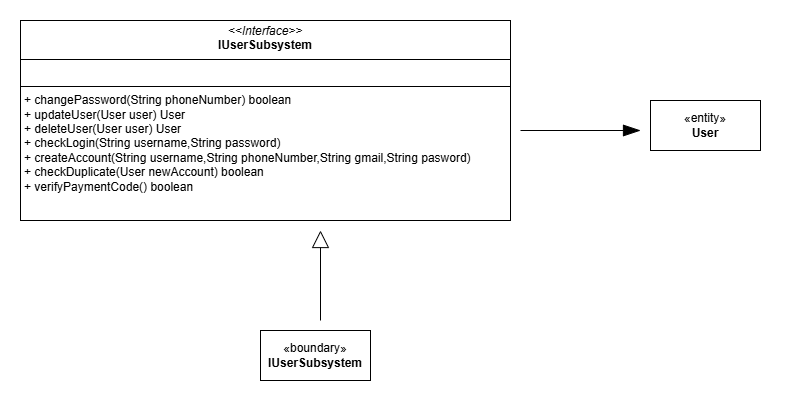
\includegraphics[width=\textwidth]{img3.1/userSubSystem(SubSystemContext).png} 
    \caption{User Subsystem Context}
\end{figure}

\begin{figure}[H]
    \centering
    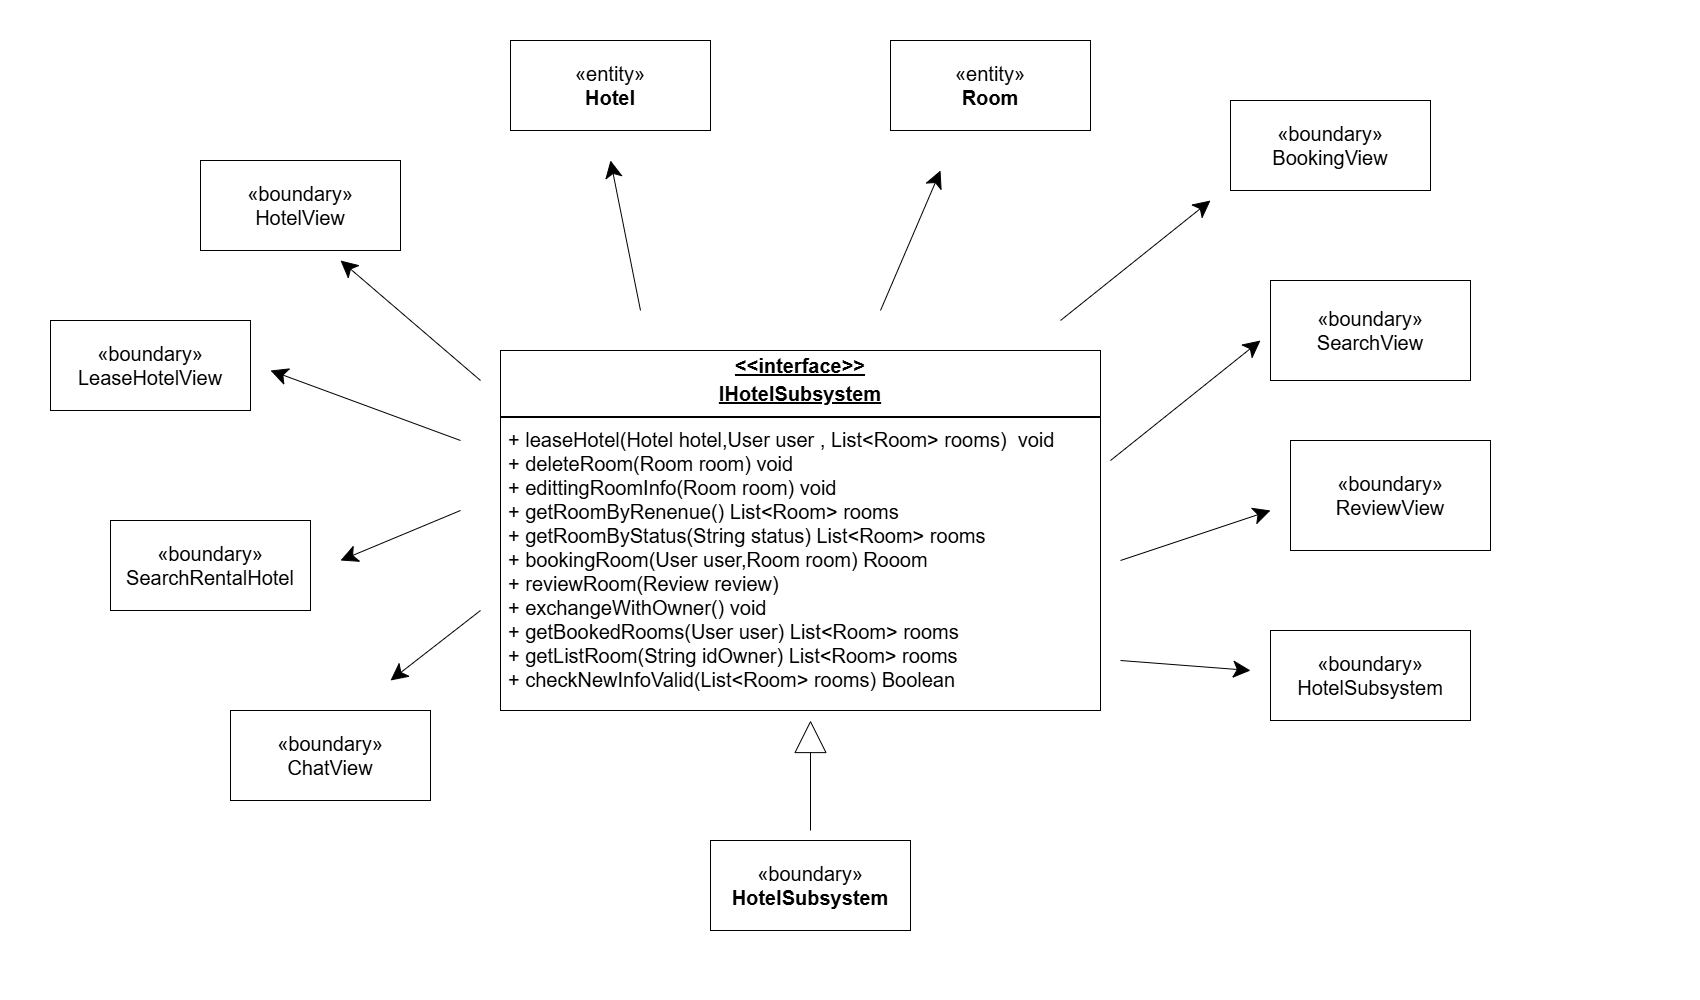
\includegraphics[width=\textwidth]{img3.1/hotelSubSystem(SubSystemContext).png}
    \caption{Hotel Subsystem Context}
\end{figure}

\begin{figure}[H]
    \centering
    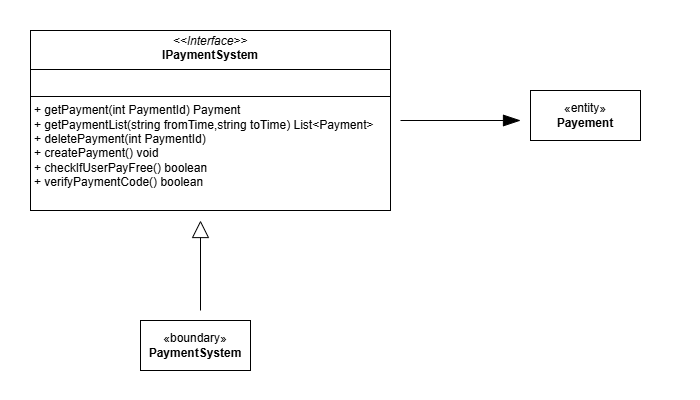
\includegraphics[width=\textwidth]{img3.1/paymentSy(SubSystemContext).png} 
    \caption{Payment Subsystem Context}
\end{figure}

\begin{figure}[H]
    \centering
    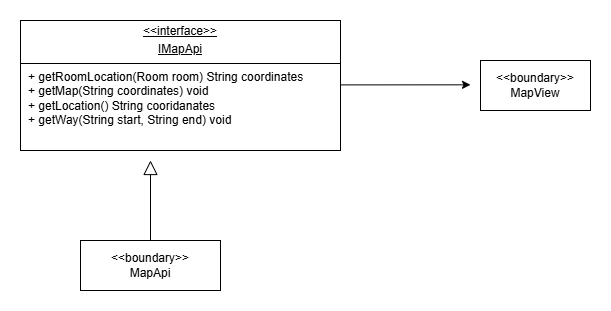
\includegraphics[width=0.9\textwidth]{img3.1/mapApi.png} 
    \caption{MapAPI System Context}
\end{figure}

\begin{figure}[H]
    \centering
    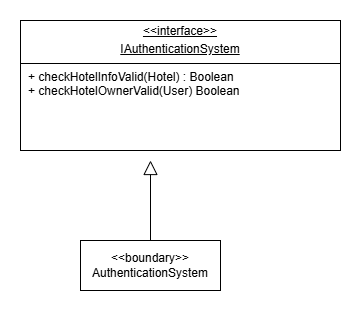
\includegraphics[width=0.9\textwidth]{img3.1/authentication.png} 
    \caption{Authentication System Context}
\end{figure}

\subsection{Analysis-to-Design-to-Implementation Mechanisms Map}
\begin{longtable}{|p{5cm}|p{4cm}|p{5cm}|}
\hline
\textbf{Cơ chế phân tích} & \textbf{Cơ chế thiết kế} & \textbf{Cơ chế cài đặt}\\
\hline
Persistency & OODBMS (new data) & ObjectStore \\
\hline
Persistency & RDBMS (data from
legacy database) & JDBC to Ingres \\
\hline
Distribution & Remote Method\newline
Invocation (RMI) & Java \\
\hline
Security & & Reverse Engineered\newline Secure.java and\newline UserContextRemoteObject components \\
\hline
Error detection/handling/reporting & & \\
\hline
\end{longtable}

\subsubsection{Cơ chế Persistency - ObjectStore OODBMS}
\textbf{Static View}
\begin{figure}[H]
    \centering
    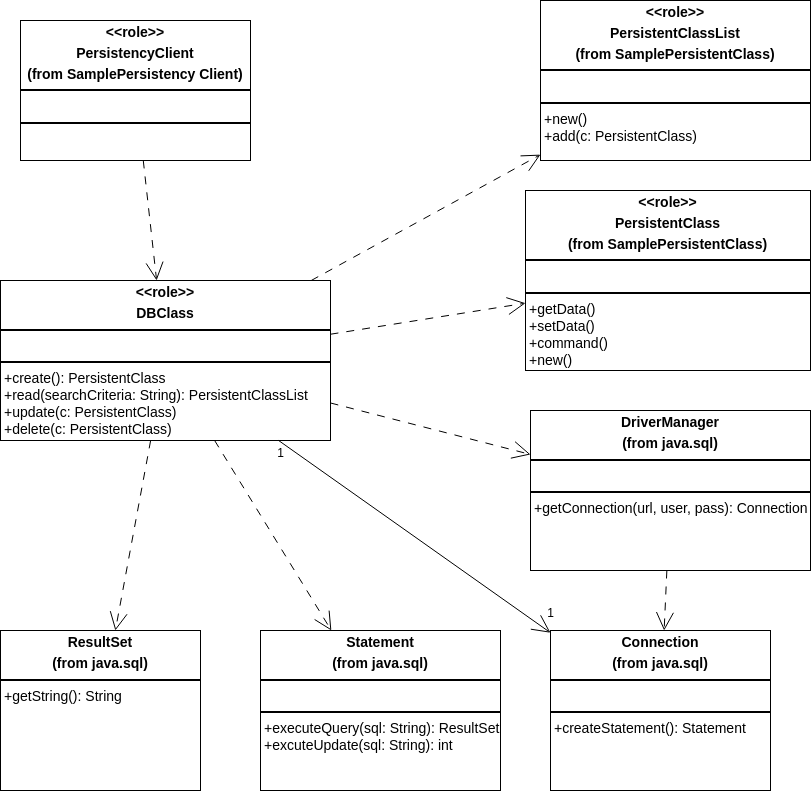
\includegraphics[width=0.95\linewidth]{img3.1.2/design mechanism-Persistency.drawio.png}
\end{figure}
\begin{itemize}
    \item Trong JDBC, một máy khách sẽ làm việc với \textbf{DBClass} để đọc và ghi dữ liệu. DBClass chịu trách nhiệm truy cập cơ sở dữ liệu JDBC bằng lớp \textbf{DriverManager}. Khi một Kết nối cơ sở dữ liệu được mở, DBClass sau đó có thể tạo các câu lệnh SQL sẽ được gửi đến RDBMS cơ bản và được thực thi bằng lớp \textbf{Statement}. Lớp Statement là lớp "nói chuyện" với cơ sở dữ liệu. Kết quả của truy vấn SQL được trả về trong một đối tượng \textbf{ResultSet}.
    \item Lớp \textbf{DBClass} chịu trách nhiệm tạo ra instnce của một lớp. Nó có cơ chế ánh xạ OO-to-RDBMS và có hành vi để giao tiếp với RDBMS. DBClass làm phẳng đối tượng, ghi nó vào RDBMS và đọc dữ liệu đối tượng từ RDBMS và xây dựng đối tượng đó. Mỗi lớp persistency sẽ có một DBClass tương ứng.
    \item \textbf{PersistentClassList} được sử dụng để trả về một tập hợp các đối tượng persistency là kết quả của truy vấn cơ sở dữ liệu.
\end{itemize}

\textbf{Dynamic View}
\begin{figure}[H]
    \centering
    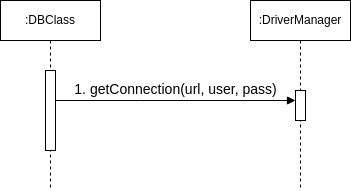
\includegraphics[width=0.75\linewidth]{img3.1.2/design mechanism-Initialize.drawio.png}
    \caption{Initialize}
\end{figure}
Bước khởi tạo phải có trước khi các lớp khác có thể kết nối. Để khởi tạo kết nối tới cơ sở dữ liệu, DBClass phải gọi hàm getConnection(). Và phương thức getConnection() sẽ tạo một kết nối với URL đã nhập sau đó trả về kết nối này.

\begin{figure}[H]
    \centering
    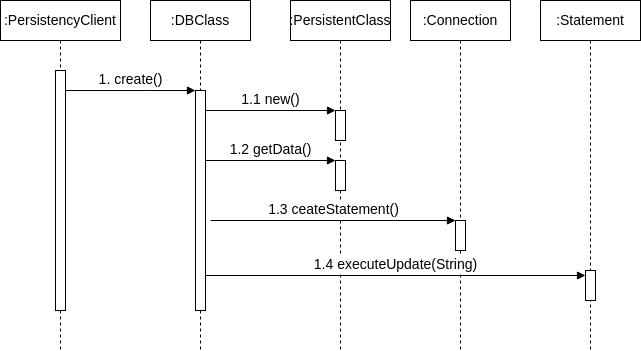
\includegraphics[width=\linewidth]{img3.1.2/design mechanism-Create.drawio.png}
    \caption{Create}
\end{figure}
Để tạo một lớp mới, DBClass tạo một thể hiện mới của PersistentClass với các giá trị mặc định. Sau đó, DBClass tạo một Statement mới bằng cách sử dụng phương thức createStatement() của lớp Connection. Statement được thực thi và dữ liệu được chèn vào cơ sở dữ liệu.

\begin{figure}[H]
    \centering
    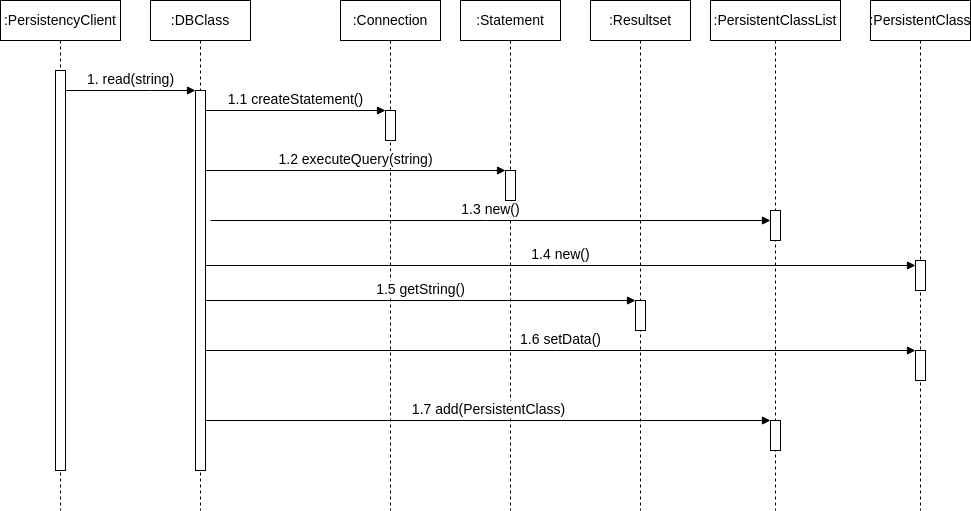
\includegraphics[width=\linewidth]{img3.1.2/design mechanism-Read.drawio.png}
    \caption{Read}
\end{figure}
Để đọc dữ liệu, DBClass tạo một Statement mới bằng cách sử dụng createStatement() của lớp Connection. Statement được thực thi và dữ liệu được trả về trong một đối tượng ResultSet. Sau đó, DBClass tạo một thể hiện mới của PersistentClass và điền vào đó dữ liệu đã truy xuất. Dữ liệu được trả về trong một đối tượng collection, một thể hiện của lớp PersistentClassList.

\begin{figure}[H]
    \centering
    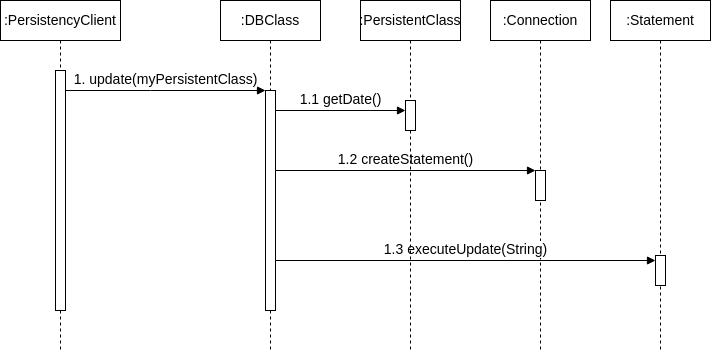
\includegraphics[width=0.9\linewidth]{img3.1.2/design mechanism-Update.drawio.png}
    \caption{Update}
\end{figure}
Để cập nhật dữ liệu, DBClass lấy dữ liệu từ đối tượng PersistentClass đã cho và tạo một Statement mới bằng cách sử dụng phương thức createStatement() của lớp Connection. Sau khi Statement được xây dựng, bản cập nhật được thực thi và cơ sở dữ liệu được cập nhật với dữ liệu mới.

\begin{figure}[H]
    \centering
    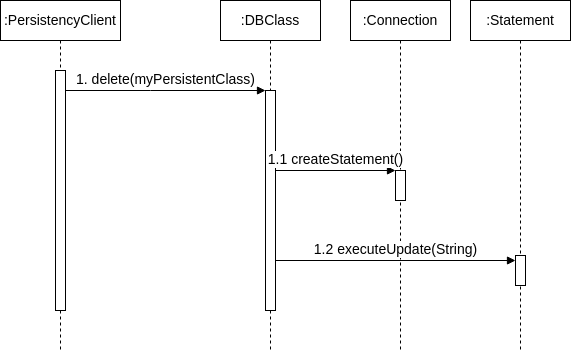
\includegraphics[width=0.9\linewidth]{img3.1.2/design mechanism-Delete.drawio.png}
    \caption{Delete}
\end{figure}
Để xóa dữ liệu, DBClass tạo một Statement mới bằng cách sử dụng phương thức createStatement() của lớp Connection. Statement được thực thi và dữ liệu được xóa khỏi cơ sở dữ liệu.

\subsubsection{Cơ chế Distribution}
\textbf{Static View}
\begin{figure}[H]
    \centering
    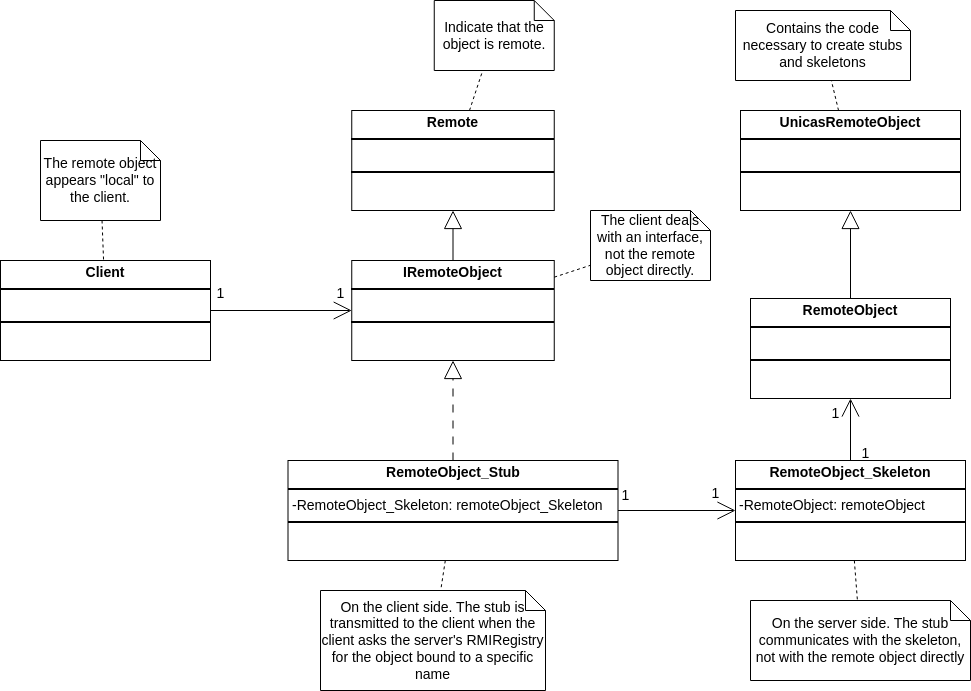
\includegraphics[width=\linewidth]{img3.1.2/design mechanism-Distribution.drawio.png}
\end{figure}

\begin{itemize}
    \item Cả client và server đều là hệ thống hướng đối tượng. Tương tác giữa server và client được đóng gói trong một hoặc nhiều đối tượng có thể truy cập từ xa. Các đối tượng này được khởi tạo trên server, nhưng client xử lý đối tượng như thể chúng là các khởi tạo cục bộ.
    \item Các stub và skeleton là các adapter, đầu tiên giúp client thích ứng với Internet và sau đó là Internet thích ứng với đối tượng của server.
    \item Bất kỳ đối tượng có thể tuần tự hóa nào đều có thể được truyền đến máy chủ bằng cách sử dụng tham số đầu vào nếu là phương thức của giao diện IRemoteObject.
    \item Bất kỳ phương thức nào mà client chạy trên đối tượng từ xa đều thực sự chạy trên server.
    \item Bất kỳ phương thức nào của đối tượng không phải UnicastRemoteObject có thể tuần tự hóa được đặt cho client đều chạy trên client.
    \item Lớp sercer phải chạy để RMIRegistry có thể tải các stub ban đầu để chuẩn bị truyền chúng tới client.
\end{itemize}

\textbf{Dynamic View}
\begin{figure}[H]
    \centering
    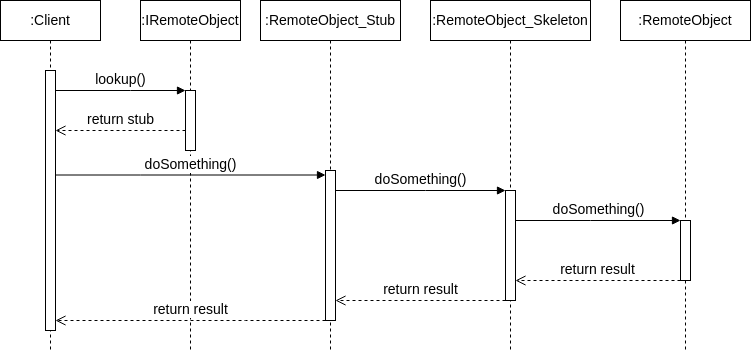
\includegraphics[width=0.9\linewidth]{img3.1.2/design mechanism-Page-8.drawio.png}
\end{figure}
\subsubsection{Cơ chế Security}
\textbf{Static View}
\begin{figure}[H]
    \centering
    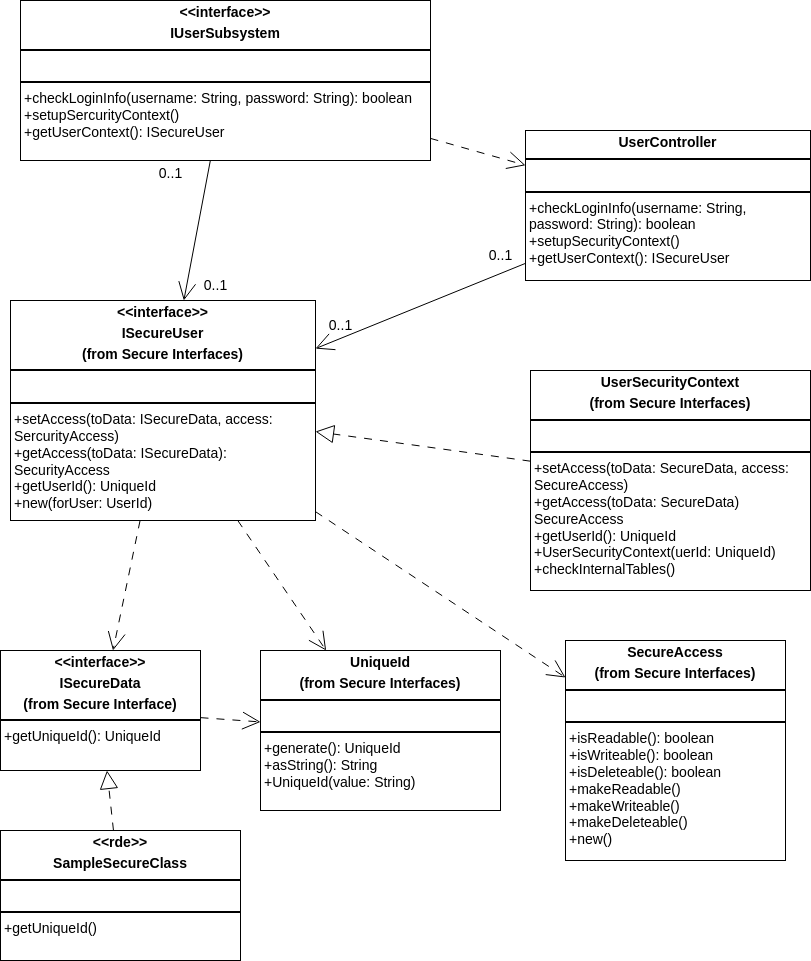
\includegraphics[width=0.8\linewidth]{img3.1.2/design mechanism-Sercurity.drawio.png}
\end{figure}
\begin{itemize}
    \item ISecureData: cơ chế phân tích: security
    \item SecurityAccess: cơ chế phân tích: security
    \item UserSecurityContext: cơ chế phân tích: security
    \item UniqueId: cơ chế phân tích: security
    \item IUserSubsystem: cơ chế phân tích: security
    \item ISecureUser: cơ chế phân tích: security
    \item UserController: cơ chế phân tích: security
\end{itemize}

\textbf{Dynamic View}
\begin{figure}[H]
    \centering
    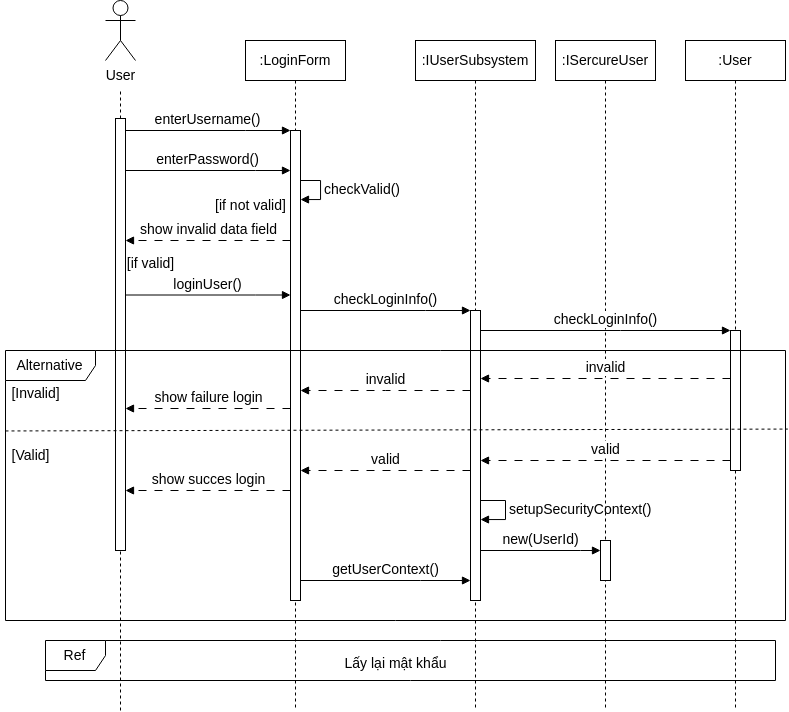
\includegraphics[width=1.1\linewidth]{img3.1.2/design mechanism-seq secure.drawio.png}
\end{figure}

\subsection{Analysis-Class-to-Design-Element Map}
\begin{longtable}{|p{6cm}|p{9cm}|}
\hline
\textbf{Analysis Class} & \textbf{Design Elements} \\
\hline
RoomSearchView & RoomSearchForm \\
\hline
RoomSearchController & RoomService \\
\hline
Room & Room \\
\hline
PaymentGateway & PaymentService \\
\hline
NotificationSystem & NotificationService\\
\hline
BookingHistoryView & BookingHistoryView \\
\hline
BookingController & BookingController, BookingRepository \\
\hline
Booking & Booking \\
\hline
BookingListView & BookingListView \\
\hline
ReviewView & ReviewView \\
\hline
ReviewController & ReviewController, ReviewRepository \\
\hline
Review & Review \\
\hline
RoomDetailView & RoomDetailView \\
\hline
ChatController & ChatController, ChatRepository \\
\hline
ChatInterface & ChatInterface \\
\hline
Message & Message,  MessageService \\
\hline
Host & Host \\
\hline
FavoriteRoomView & FavoriteRoomView \\
\hline
FavoriteController & FavoriteController, FavorieRepository \\
\hline
Room & Room \\
\hline
UserController & UserController \\
\hline
LeaseHotelView & LeaseHotelView \\
\hline
AuthenticationSystem & AuthenticationSystem \\
\hline
LeaseHotelController & LeaseHotelController \\
\hline
HotelDatabase & HotelDatabase \\
\hline
HotelView & HotelView \\
\hline
HotelController & HotelController, IHotelSubSystem \\
\hline
SearchRentalHotelView & SearchRentalHotelView \\
\hline
SearchRentalHotelController & SearchRentalHotelController \\
\hline
PaymentView & PaymentView \\
\hline
PaymentController & PaymentController \\
\hline
Payment & Payment \\
\hline
PaymentSystem & IPaymentSystem \\
\hline
OrderView & OrderView \\
\hline
OrderController & OrderController, IOrderSystem \\
\hline
Order & Order \\
\hline
FindVehicleView & FindVehicleView \\
\hline
FindVehicleController & FindVehicleController \\
\hline
LeaseHotelController & LeaseHotelController \\
\hline
AuthenticationSystem & IAuthentifacationSubSystem\\
\hline
MapAPISystem & ImapAPI \\
\hline
RegisterForm & RegisterForm \\
\hline
UserDatabase & UserDatabase \\
\hline
User & User, IUserSubsystem \\
\hline
LoginForm & LoginForm \\
\hline
NewPasswordForm & NewPasswordForm \\
\hline
ChangeInfoForm & ChangeInfoForm \\
\hline
DeleteAccountForm &DeleteAccountForm \\
\hline
LanguageView & LanguageView \\
\hline
LanguageController & LanguageController \\
\hline
\end{longtable}

\subsection{Design-Element-to-Owning-Package Map}
\begin{longtable}{|p{6cm}|p{9cm}|}
\hline
\textbf{Design Elements
Owni} & \textbf{Owning package} \\
\hline
RoomSearchForm & GUI\_Management \\
\hline
RoomService & Subsystem.HotelSubsystem \\
\hline
Room & Database.Hotelinfo \\
\hline
PaymentService & Subsystem.PaymentSystem \\
\hline
NotificationService & Subsystem \\
\hline
BookingHistoryView & GUI\_Management \\
\hline
BookingController & Subsystem.BookingSubsystem \\
\hline
BookingRepository & Subsystem.BookingSubsystem \\
\hline
Booking & Database.Bookingdata\\
\hline
BookingListView & GUI\_Management \\
\hline
ReviewView & GUI\_Management \\
\hline
ReviewController & Database.ReviewSubsystem \\
\hline
ReviewRepository & Subsystem.ReviewSubsystem \\
\hline
Review & Database.Reviewdata \\
\hline
RoomDetailView & GUI\_Management \\
\hline
ChatController & Subsystem.ChatSubsystem \\
\hline
ChatRepository & Subsystem.ChatSubsystem \\
\hline
ChatInterface &  Subsystem.ChatSubsystem\\
\hline
Message & Database.Bookingdata\\
\hline
MessageService & Subsystem.ChatSubsystem \\
\hline
Host & Database.Userdata \\
\hline
FavoriteRoomView & GUI\_Management \\
\hline
FavoriteController & Subsystem.BookingSubsystem \\ 
\hline
FavorieRepository & Subsystem.BookingSubsystem \\
\hline
Room & Database.hoteldata \\
\hline
UserController & Subsystem.UserSubsystem \\
\hline
LeaseHotelView & GUI\_Management \\
\hline
AuthenticationSystem & Subsystem \\
\hline
LeaseHotelController & Subsystem.BookingSubsystem \\
\hline
HotelDatabase & Database.Hoteldata \\
\hline
HotelView & GUI\_Management \\
\hline
HotelController & Subsystem.HotelSubsystem \\
\hline
IHotelSubSystem & Subsystem.HotelSubsystem \\
\hline
SearchRentalHotelView & GUI\_Management \\
\hline
SearchRentalHotelController & Subsystem.BookingSubsystem \\
\hline
PaymentView & GUI\_Management \\
\hline
PaymentController & Subsystem.PaymentSystem \\
\hline
Payment & Database.Bookingdata \\
\hline
PaymentSystem & Subsystem.PaymentSystem \\
\hline
OrderView & GUI\_Management \\
\hline
OrderController & Subsystem.BookingSubsystem \\
\hline
IOrderSystem & Subsystem.BookingSubsystem \\
\hline
Order & Database.Bookingdata \\
\hline
FindVehicleView & GUI\_Management \\
\hline
FindVehicleController & Subsystem.BookingSubsystem \\
\hline
LeaseHotelController & Subsystem.BookingSubsystem \\
\hline
AuthenticationSystem & Subsystem\\
\hline
MapAPISystem & GUI\_Management \\
\hline
RegisterForm & GUI\_Management \\
\hline
UserDatabase & Database.Userdata \\
\hline
User & Database.Userdata\\ 
\hline
IUserSubsystem & Subsystem.UserSubsystem \\
\hline
LoginForm & GUI\_Management \\
\hline
NewPasswordForm & GUI\_Management \\
\hline
ChangeInfoForm & GUI\_Management \\
\hline
DeleteAccountForm & GUI\_Management \\
\hline
LanguageView & GUI\_Management \\
\hline
LanguageController & Subsystem \\
\hline
\end{longtable}

\subsection{Packages and Their Dependency}
\begin{figure}[H]
    \centering
    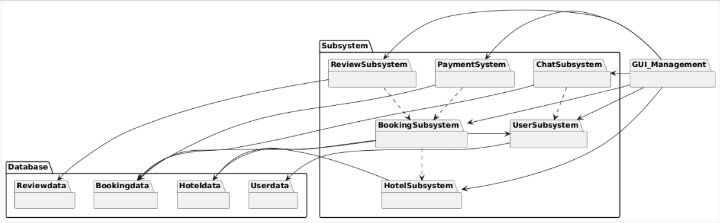
\includegraphics[width=\textwidth]{img3.1.5/Blank 2 Grids Collage_0.jpg} 
\end{figure}

\section{Mô tả kiến trúc thực thi}
\begin{figure}[H]
    \centering
    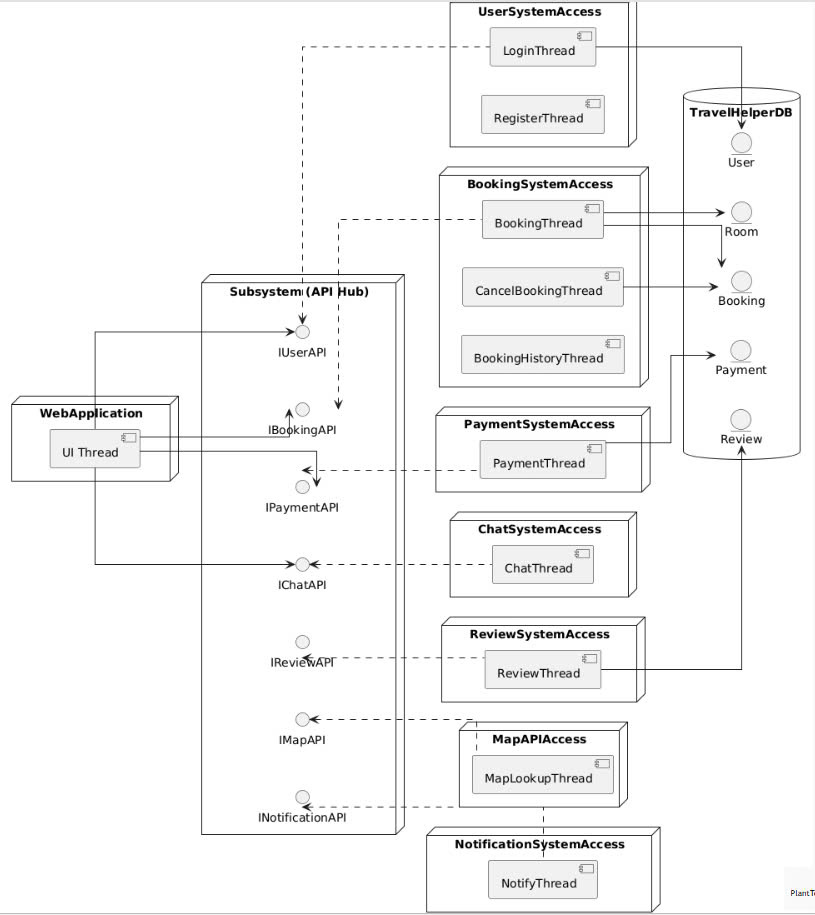
\includegraphics[width=\linewidth]{img3.2/1.jpg}
\end{figure}

\section{Thiết kế Use Case }

\subsection{Thiết kế biểu đồ tuần tự}
\subsubsection{Đặt phòng khách sạn}
\begin{figure}[H]
    \centering
    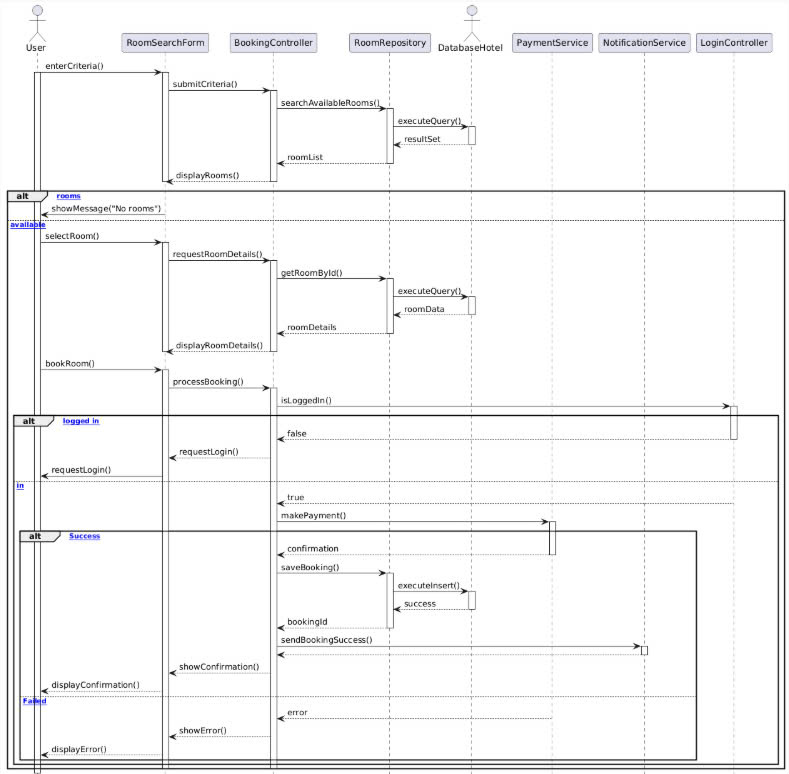
\includegraphics[width=\textwidth]{img3.4/timphong3.jpg} 
    \caption{Biểu đồ tuần tự Đặt phòng khách sạn}
\end{figure}

\subsubsection{Theo dõi phòng đã đặt}
\begin{figure}[H]
    \centering
    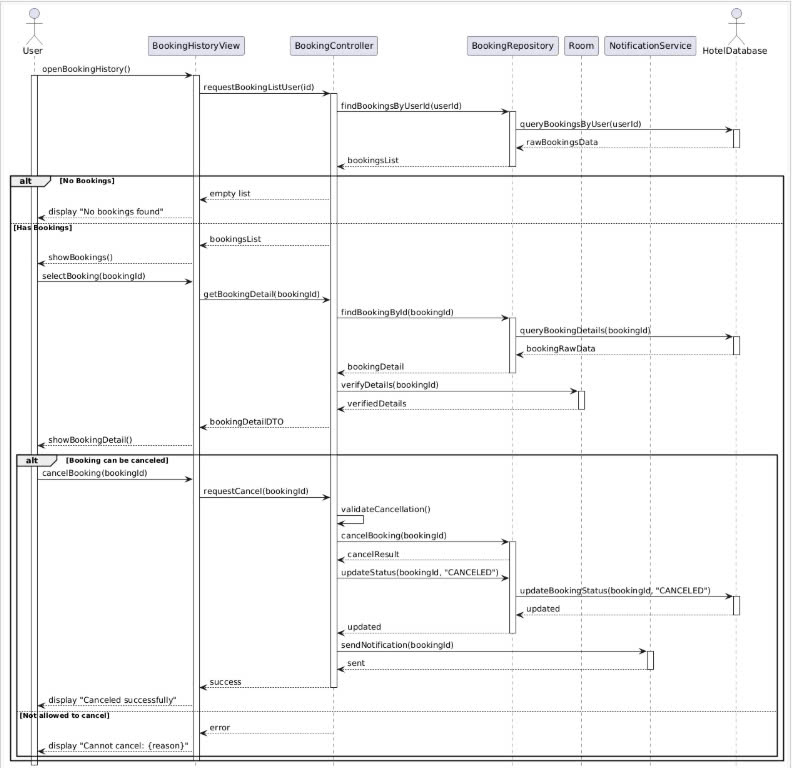
\includegraphics[width=\textwidth]{img3.4/xemphongthue3.jpg} 
    \caption{Biểu đồ tuần tự Theo dõi phòng đã đặt}
\end{figure}

\subsubsection{Đánh giá phòng đã thuê}
\begin{figure}[H]
    \centering
    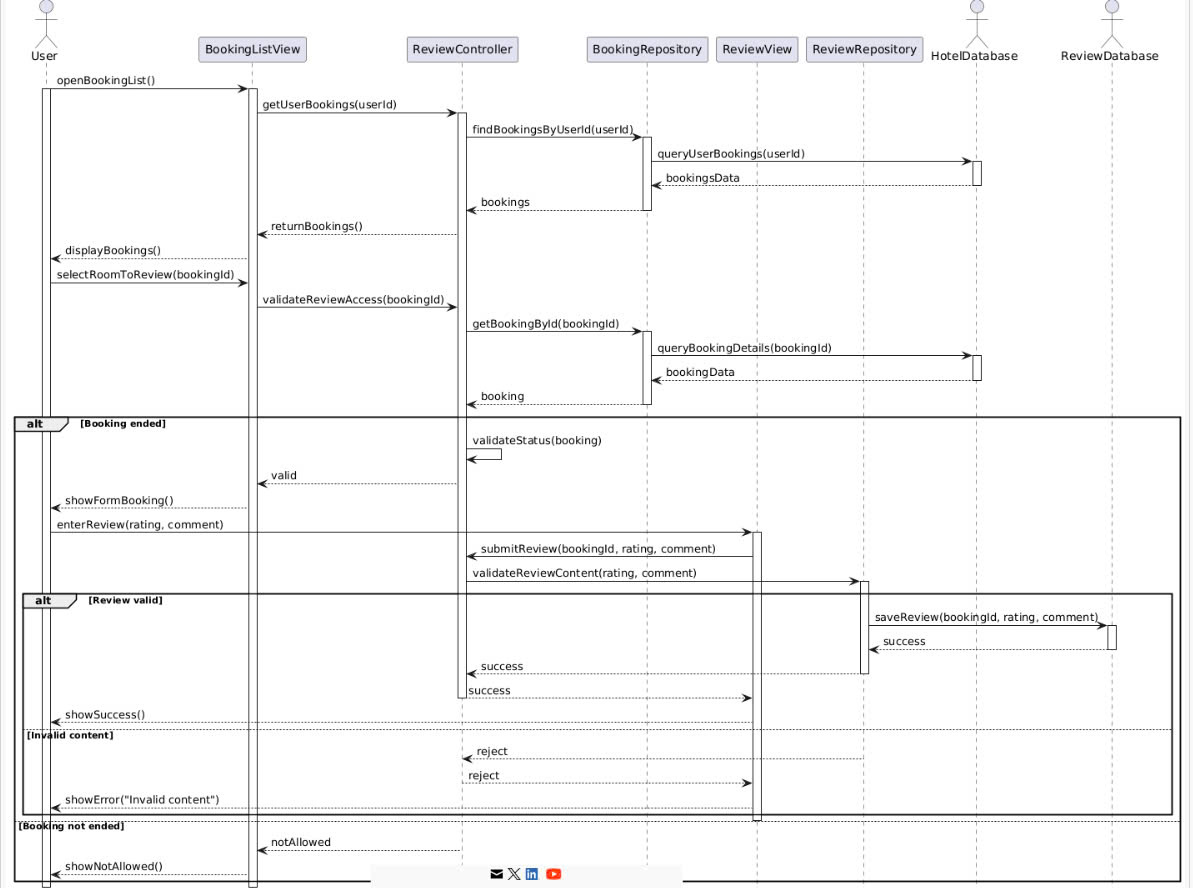
\includegraphics[width=\textwidth]{img3.4/dgia3.jpg} 
    \caption{Biểu đồ tuần tự Đánh giá phòng đã thuê}
\end{figure}

\subsubsection{Liên hệ với chủ khách sạn}
\begin{figure}[H]
    \centering
    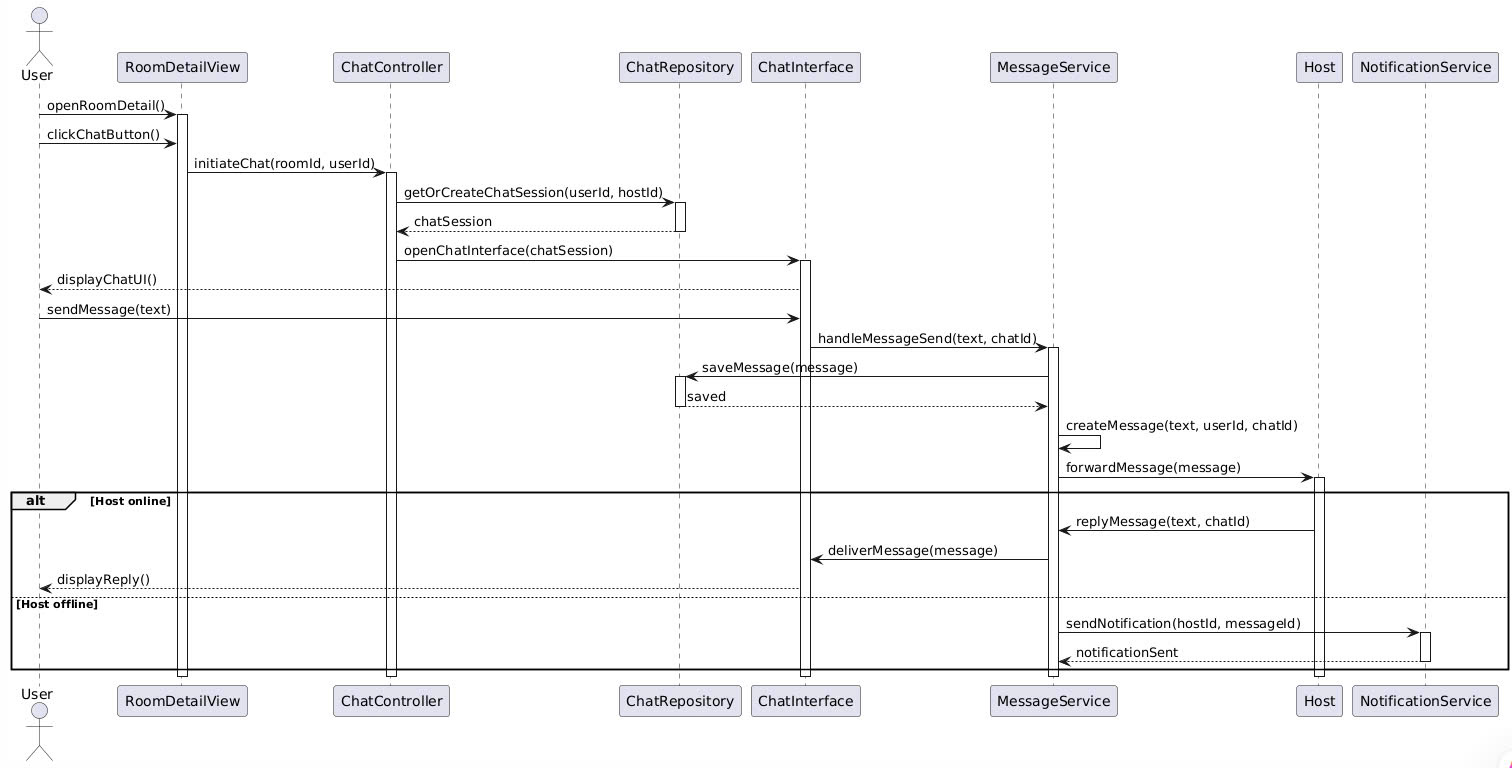
\includegraphics[width=\textwidth]{img3.4/chat3.jpg} 
    \caption{Biểu đồ tuần tự Liên hệ với chủ khách sạn}
\end{figure}

\subsubsection{Xem danh sách phòng yêu thích}
\begin{figure}[H]
    \centering
    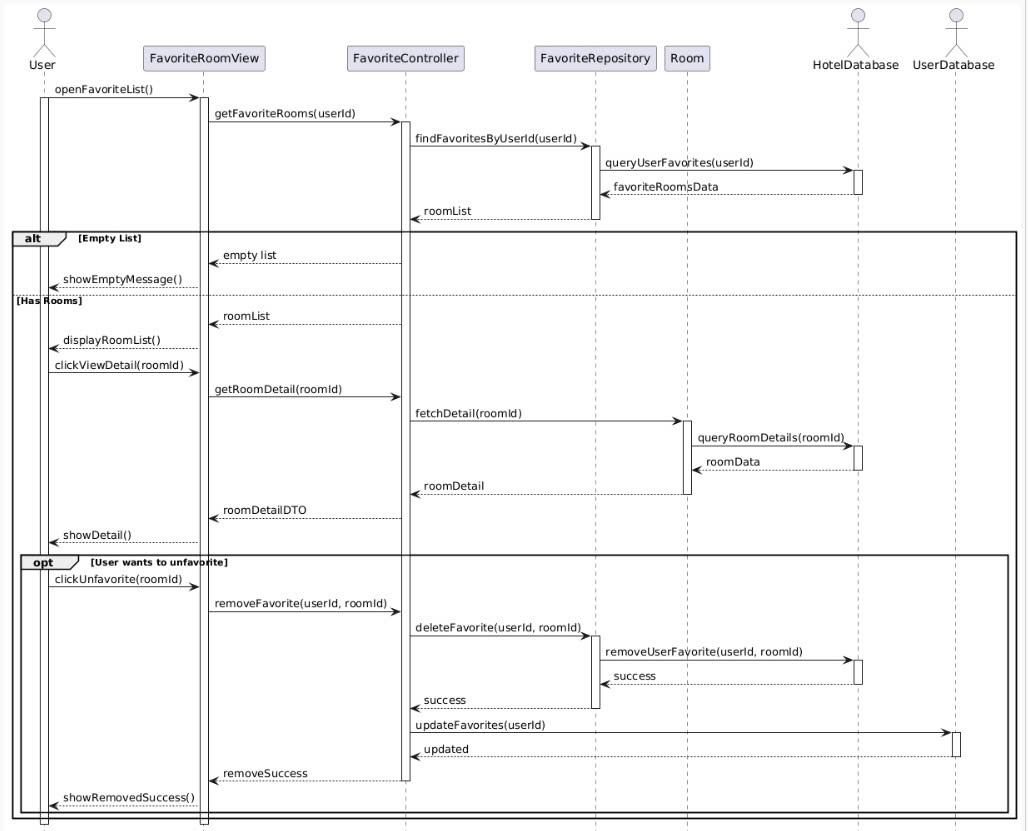
\includegraphics[width=\textwidth]{img3.4/xemphongyeu3.jpg} 
    \caption{Biểu đồ tuần tự Xem danh sách phòng yêu thích}
\end{figure}

\subsubsection{Cho thuê phòng}
\begin{figure}[H]
    \centering
    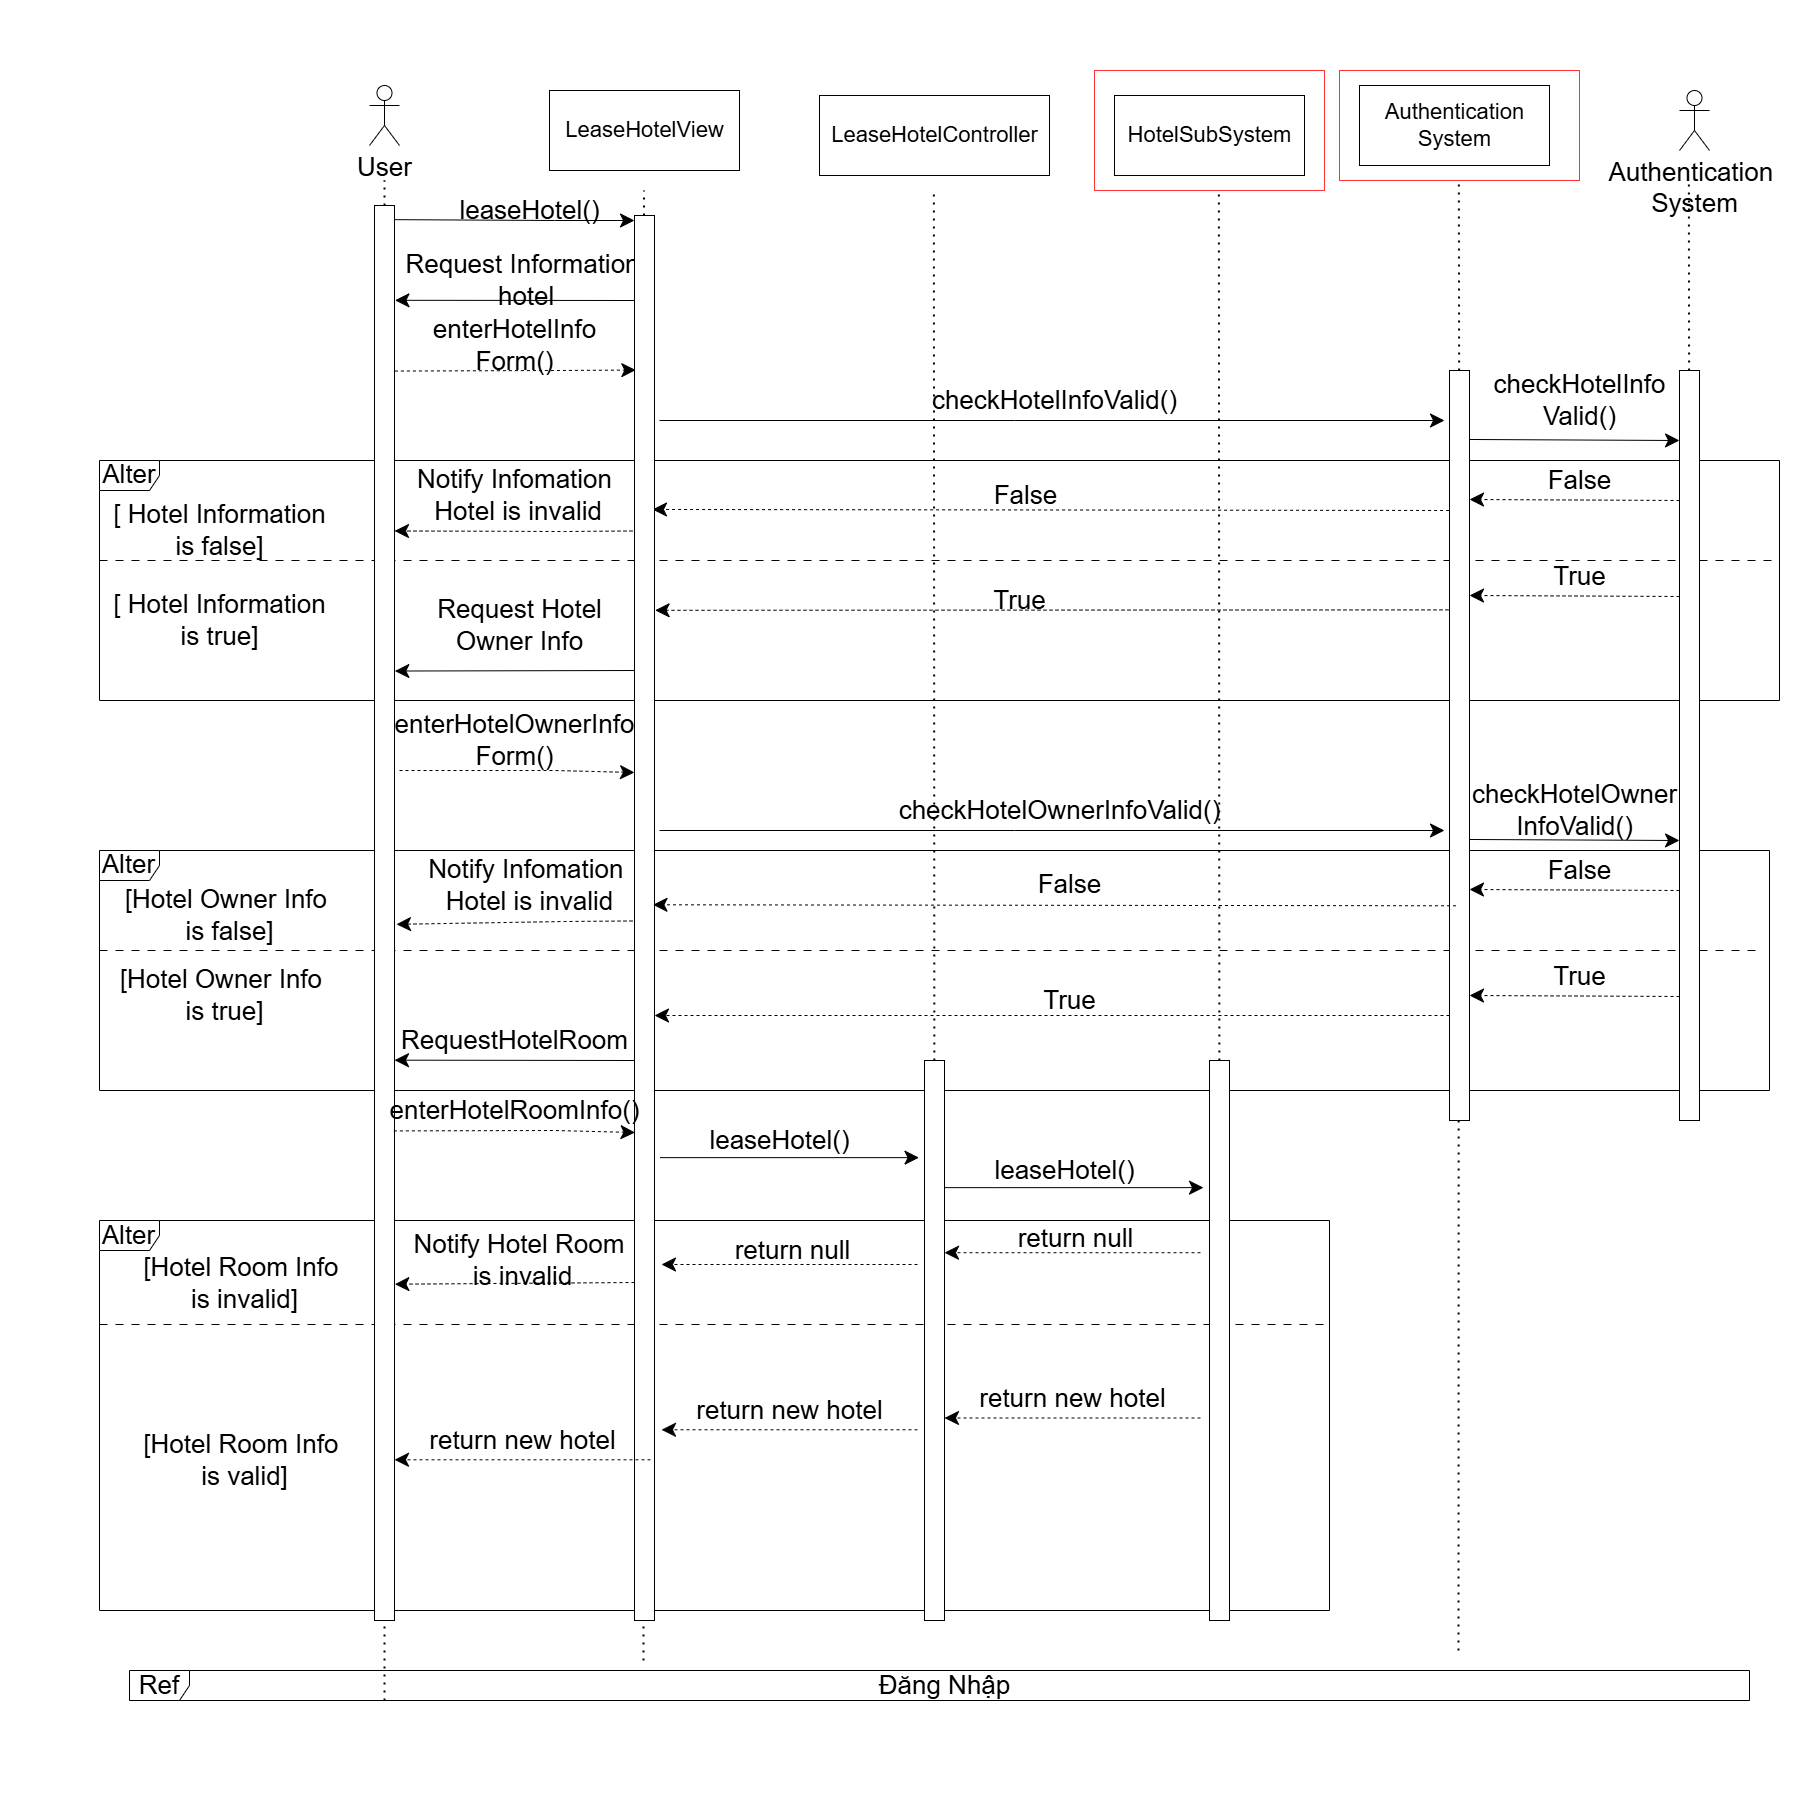
\includegraphics[width=\textwidth]{img3.4/chothuephong.png} 
    \caption{Biểu đồ tuần tự Cho thuê phòng}
\end{figure}

\subsubsection{Sửa thông tin phòng}
\begin{figure}[H]
    \centering
    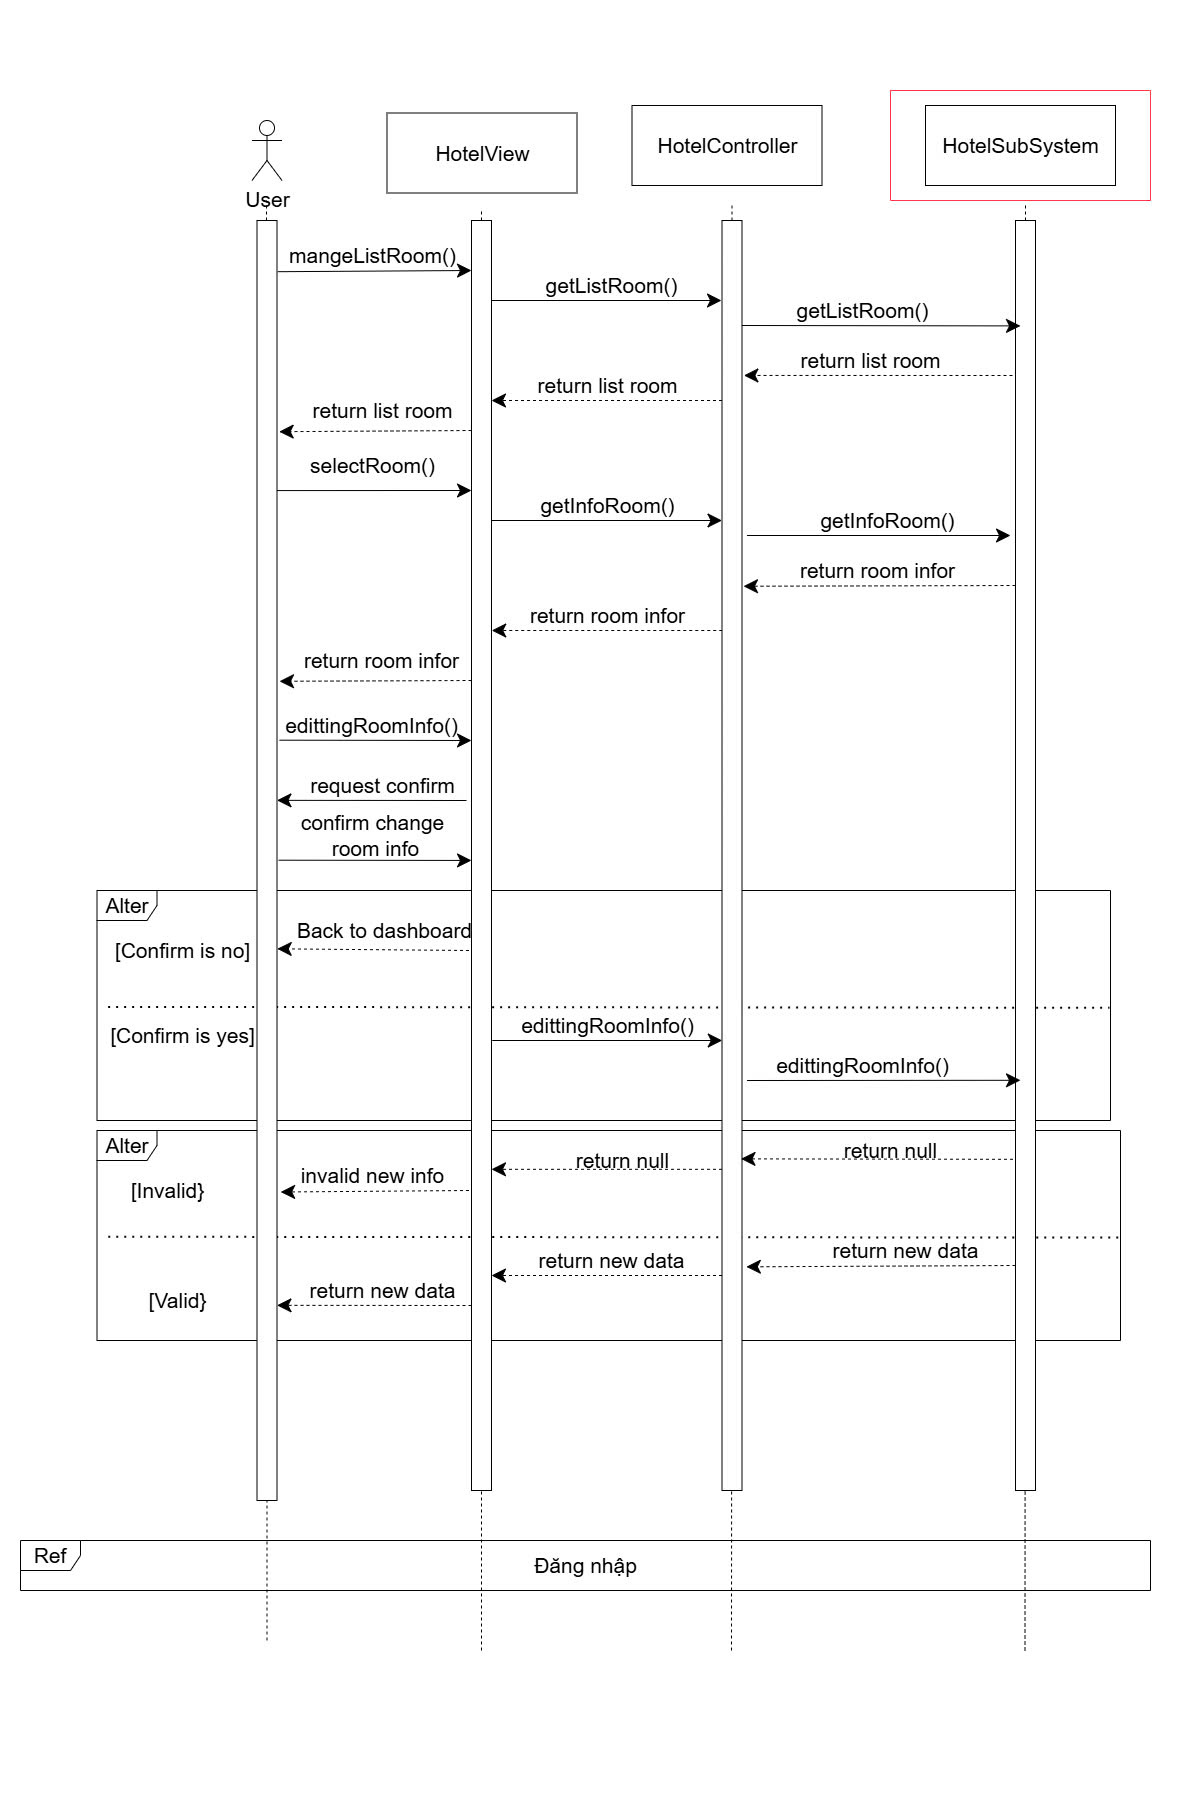
\includegraphics[width=0.75\textwidth]{img3.4/doitrangthaiphong.jpg} 
    \caption{Biểu đồ tuần tự Sửa thông tin phòng}
\end{figure}

\subsubsection{Tra cứu thông tin phòng đang cho thuê}
\begin{figure}[H]
    \centering
    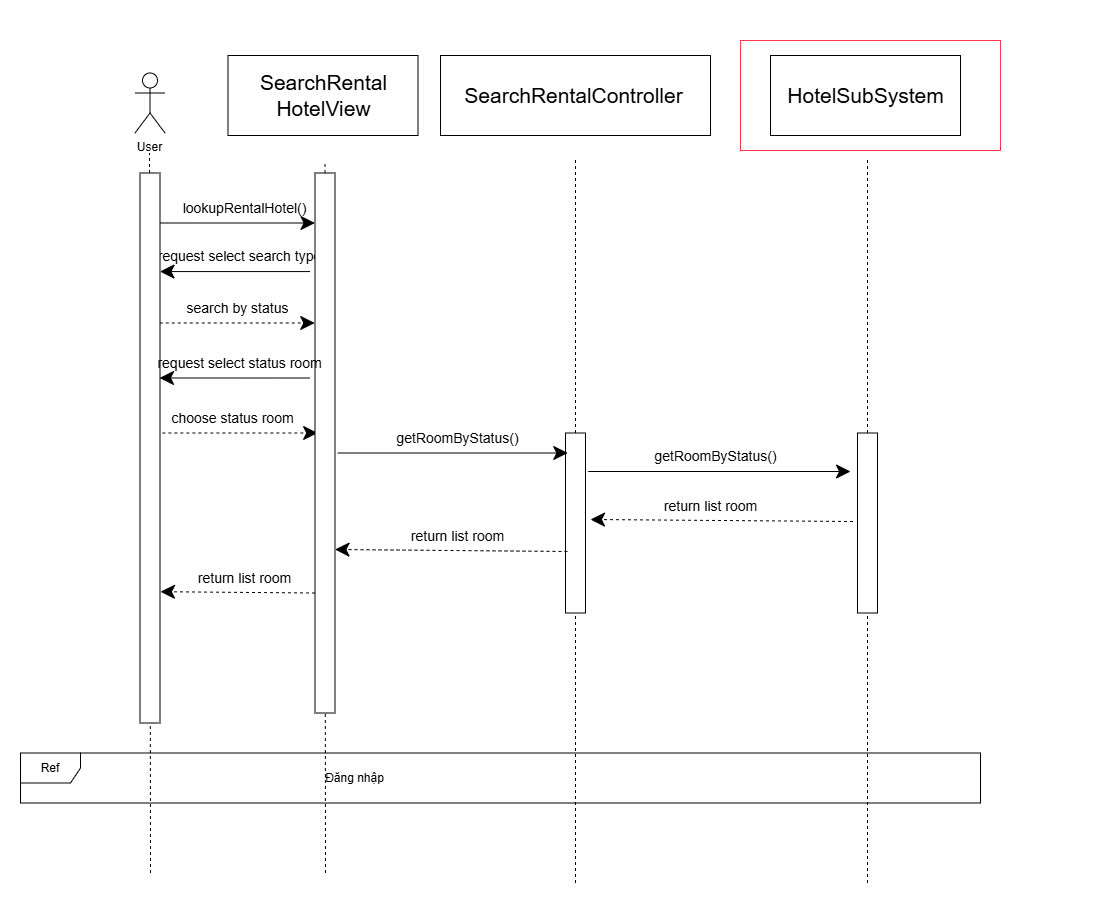
\includegraphics[width=\textwidth]{img3.4/tracuutheotrangthai.jpg} 
    \caption{Biểu đồ tuần tự Tra cứu phòng theo trạng thái}
\end{figure}

\begin{figure}[H]
    \centering
    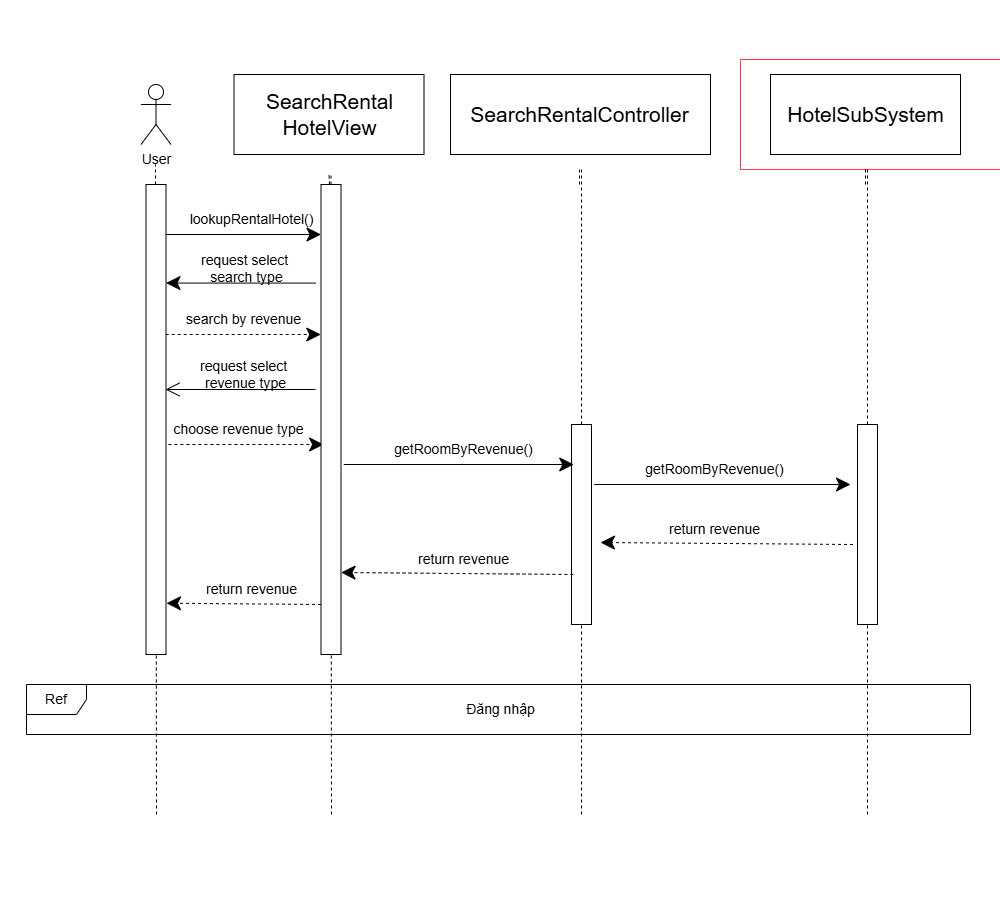
\includegraphics[width=\textwidth]{img3.4/tracuutheodoanhthu.jpg} 
    \caption{Biểu đồ tuần tự Tra cứu doanh thu phòng}
\end{figure}

\subsubsection{Xóa phòng khách sạn}
\begin{figure}[H]
    \centering
    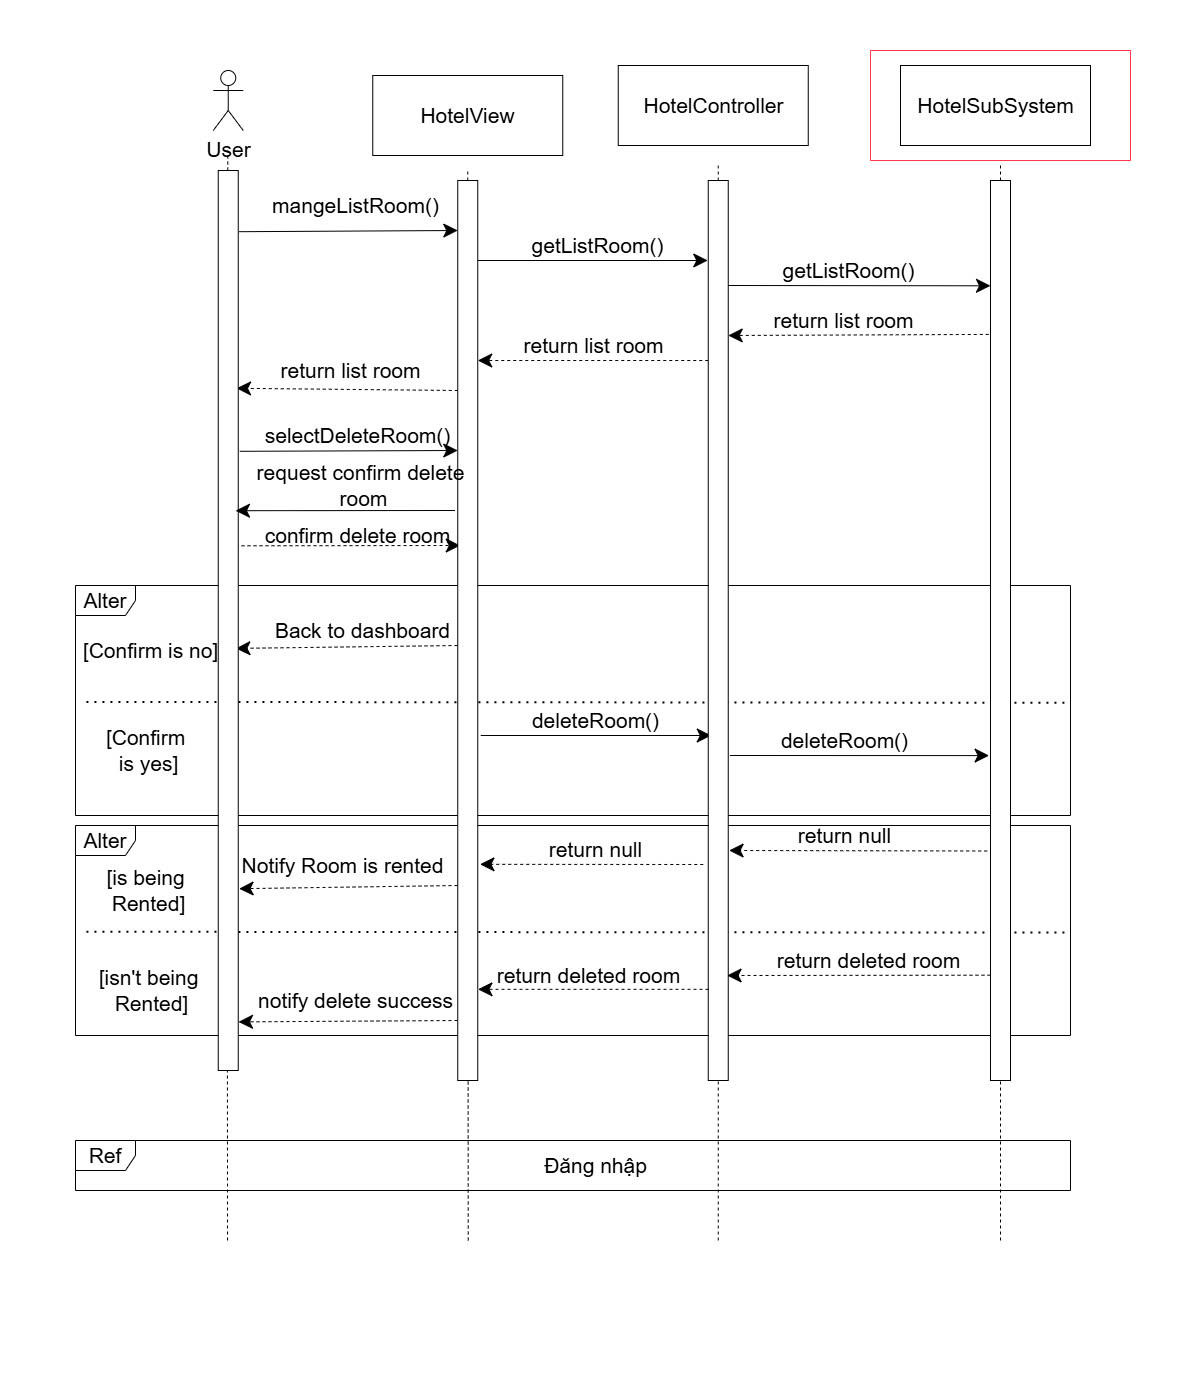
\includegraphics[width=0.95\textwidth]{img3.4/xoaphong.jpg} 
    \caption{Biểu đồ tuần tự Xóa phòng khách sạn}
\end{figure}

\subsubsection{Thanh toán}
\begin{figure}[H]
    \centering
    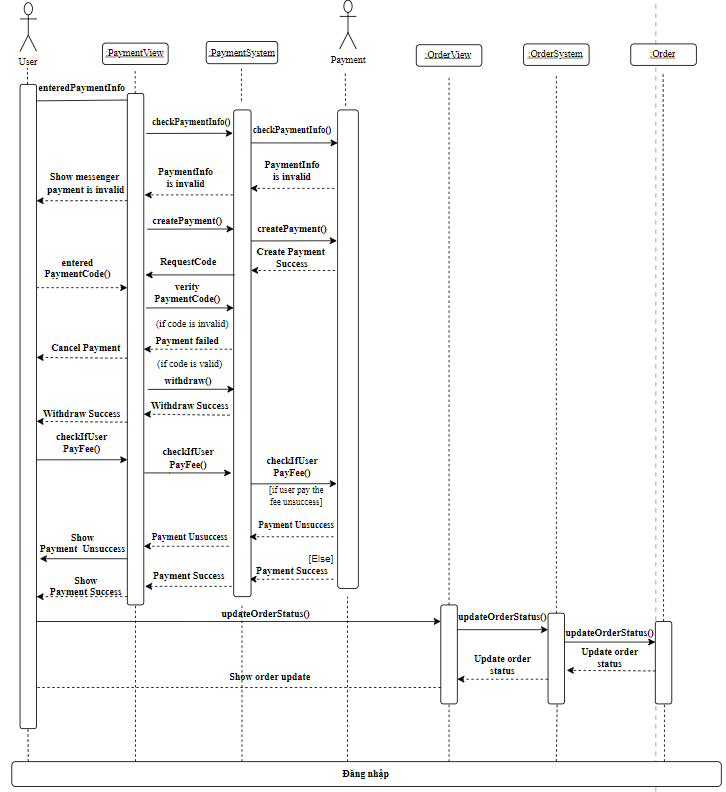
\includegraphics[width=\textwidth]{img3.4/3.4.1thanhtoanbangtk.png} 
    \caption{Biểu đồ tuần tự Thanh toán trực tuyến}
\end{figure}

\begin{figure}[H]
    \centering
    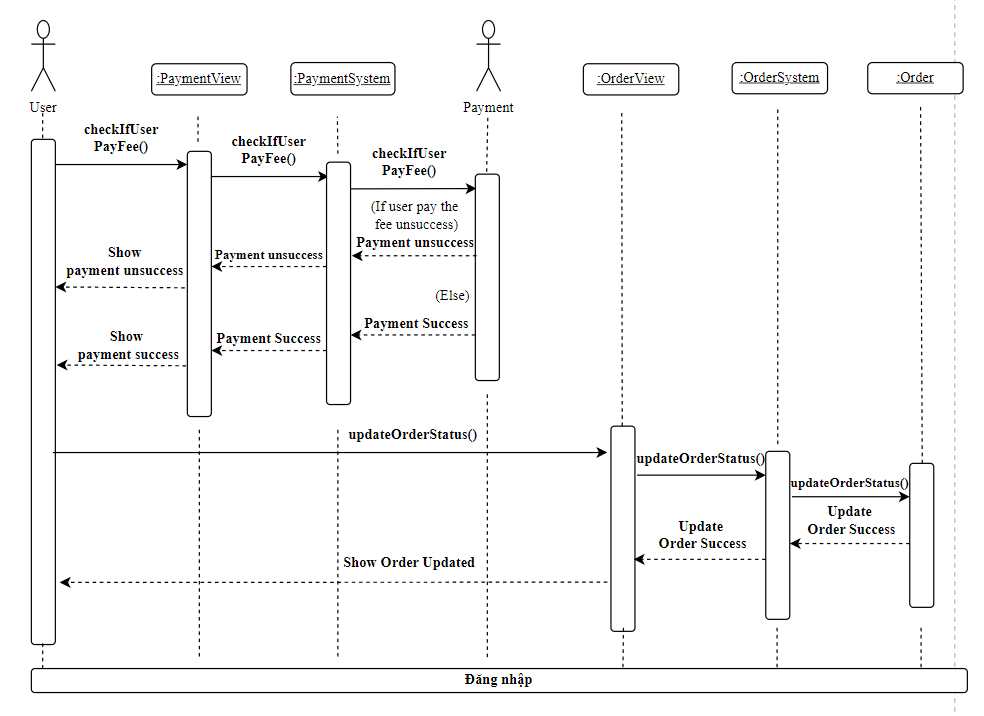
\includegraphics[width=\textwidth]{img3.4/3.4.1thanhtoantructiep.png} 
    \caption{Biểu đồ tuần tự Thanh toán trực tiếp}
\end{figure}

\subsubsection{Tra cứu phương tiện}
\begin{figure}[H]
    \centering
    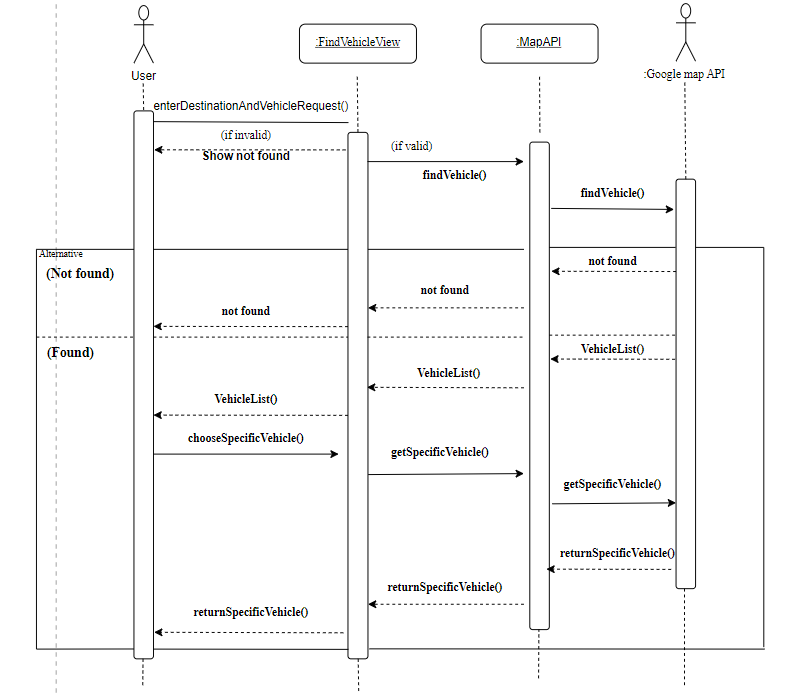
\includegraphics[width=\textwidth]{img3.4/3.4.1 timphuongtien.png} 
    \caption{Biểu đồ tuần tự Tra cứu phương tiện}
\end{figure}

\subsubsection{Đăng ký tài khoản}
\begin{figure}[H]
    \centering
    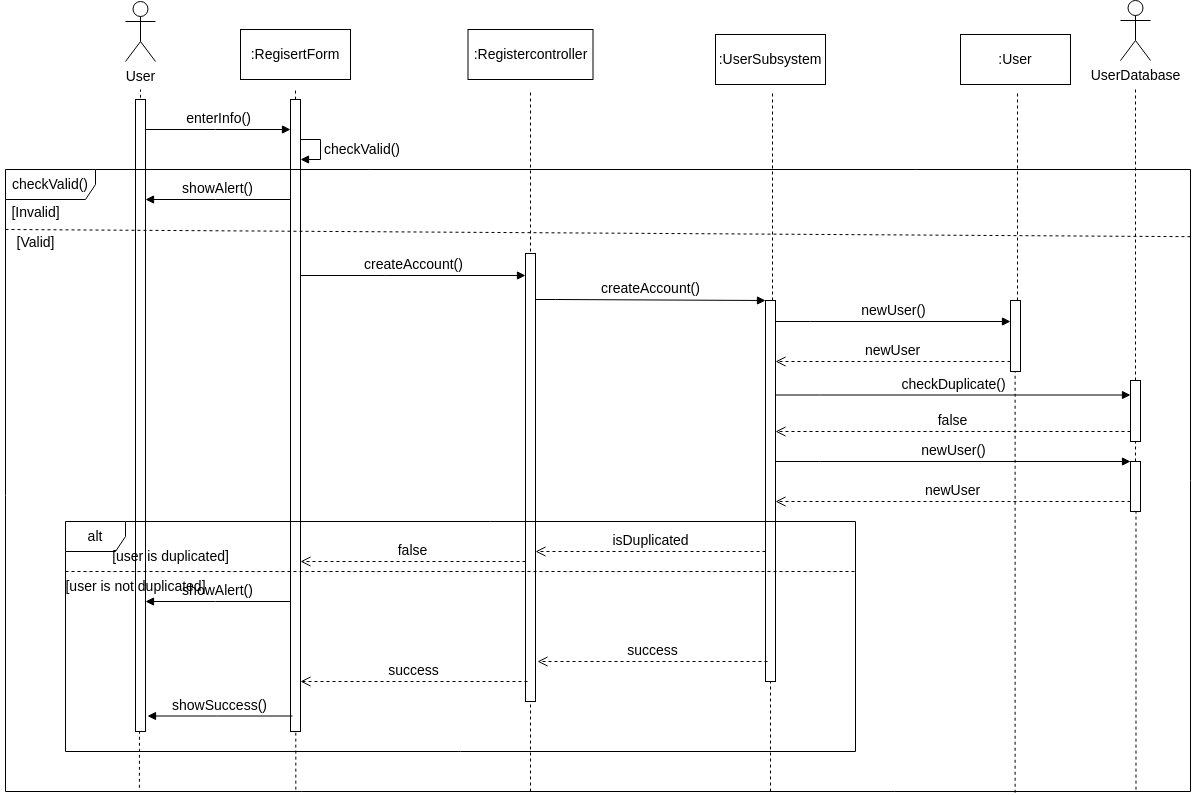
\includegraphics[width=\textwidth]{img3.4/Design_diagram-Đăng ký.drawio.png} 
    \caption{Biểu đồ tuần tự Đăng ký tài khoản}
\end{figure}

\subsubsection{Đăng nhập}
\begin{figure}[H]
    \centering
    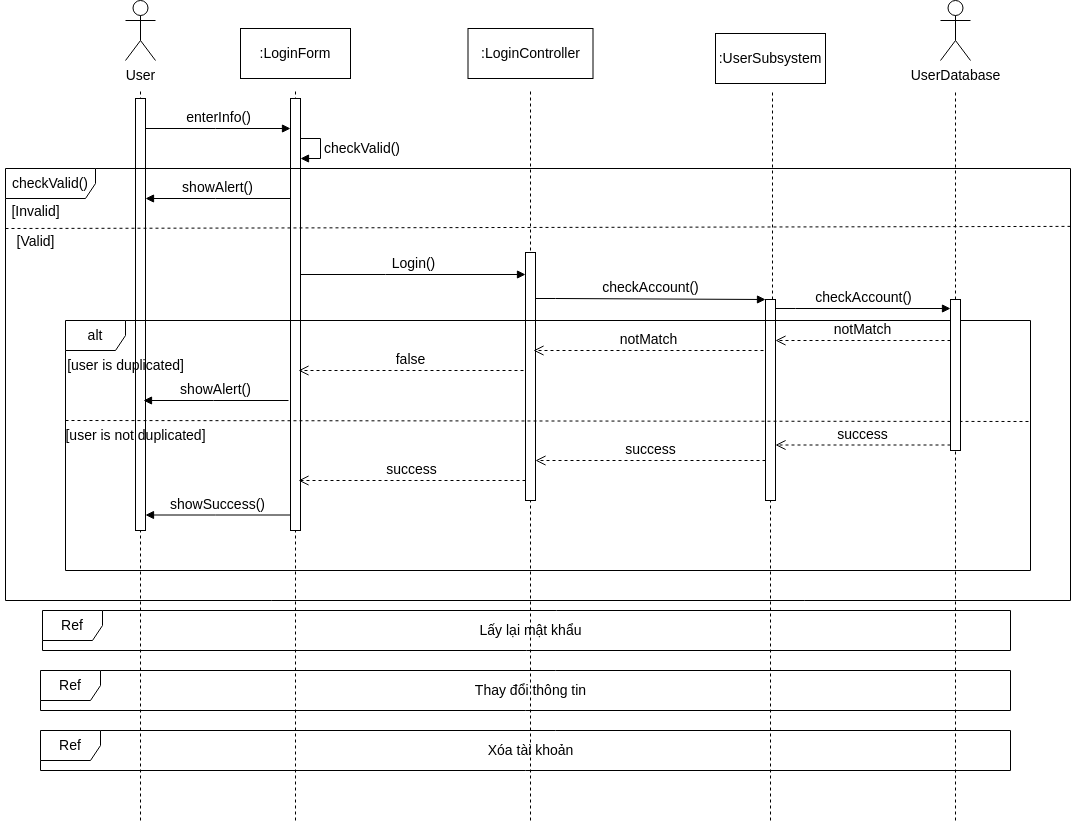
\includegraphics[width=\textwidth]{img3.4/Design_diagram-Đăng nhập.drawio.png} 
    \caption{Biểu đồ tuần tự Đăng nhập}
\end{figure}

\begin{figure}[H]
    \centering
    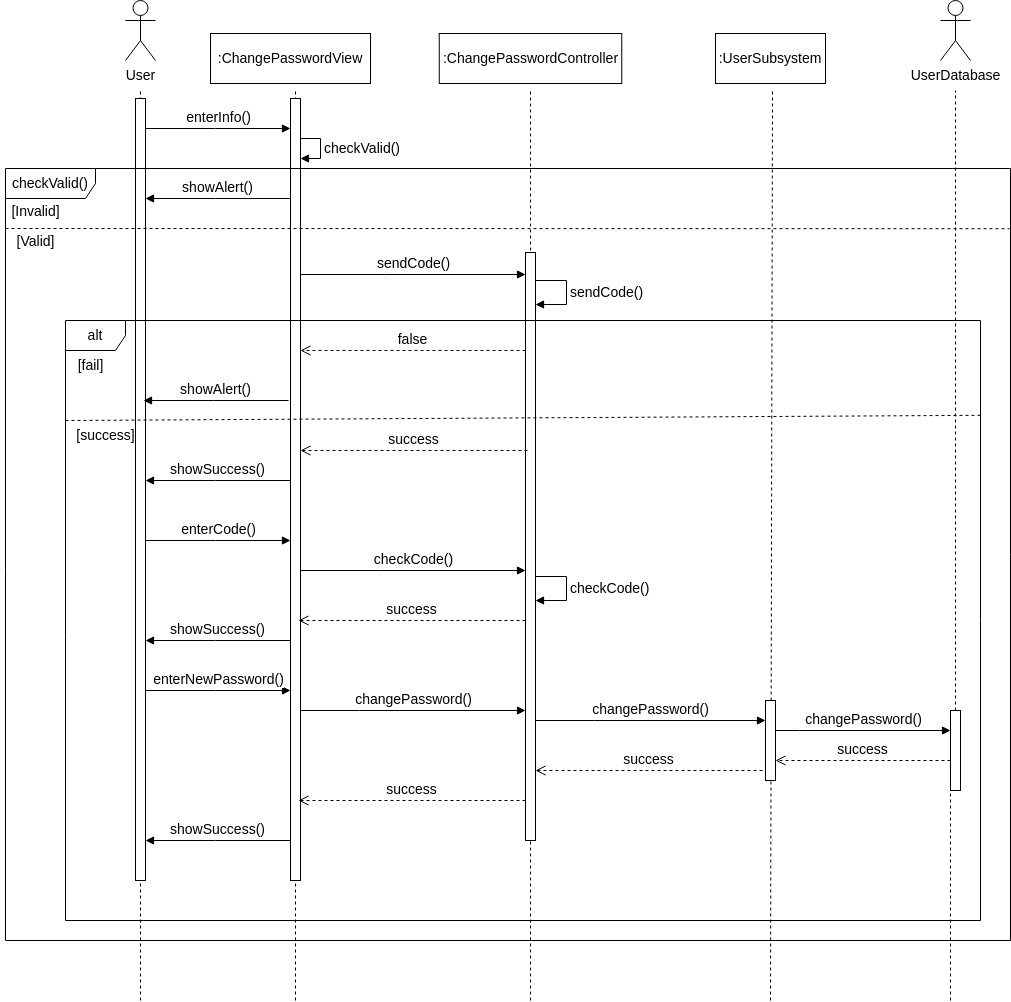
\includegraphics[width=\textwidth]{img3.4/Design_diagram-Quên mật khẩu.drawio.png} 
    \caption{Biểu đồ tuần tự Quên mật khẩu}
\end{figure}

\begin{figure}[H]
    \centering
    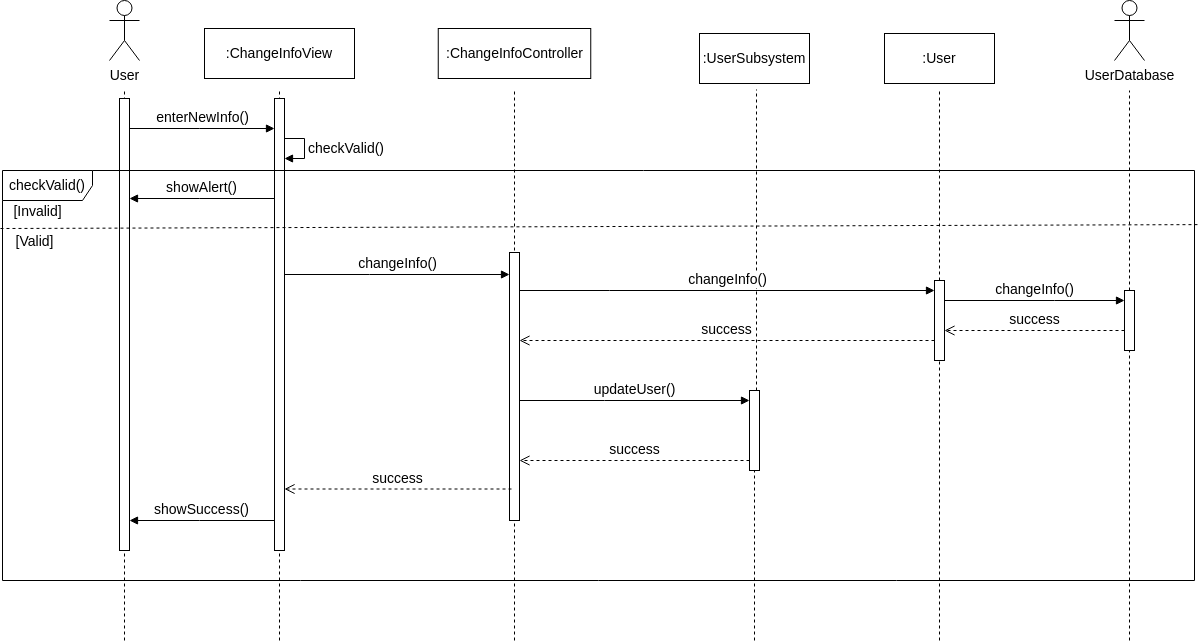
\includegraphics[width=\textwidth]{img3.4/Design_diagram-Thay đổi thông tin.drawio.png} 
    \caption{Biểu đồ tuần tự Thay đổi thông tin tài khoản}
\end{figure}

\begin{figure}[H]
    \centering
    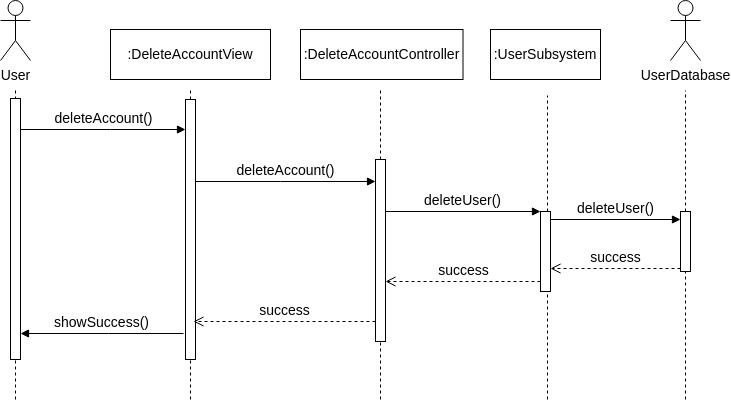
\includegraphics[width=\textwidth]{img3.4/Design_diagram-Xóa tài khoản.drawio.png} 
    \caption{Biểu đồ tuần tự Xóa tài khoản}
\end{figure}

\subsubsection{Lựa chọn ngôn ngữ}
\begin{figure}[H]
    \centering
    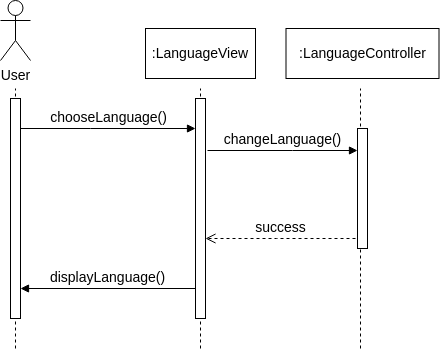
\includegraphics[width=\textwidth]{img3.4/Design_diagram-Chọn ngôn ngữ.drawio.png} 
    \caption{Biểu đồ tuần tự Lựa chọn ngôn ngữ}
\end{figure}

\subsection{Thiết kế biểu đồ lớp}
\subsubsection{Đặt phòng khách sạn}
\begin{figure}[H]
    \centering
    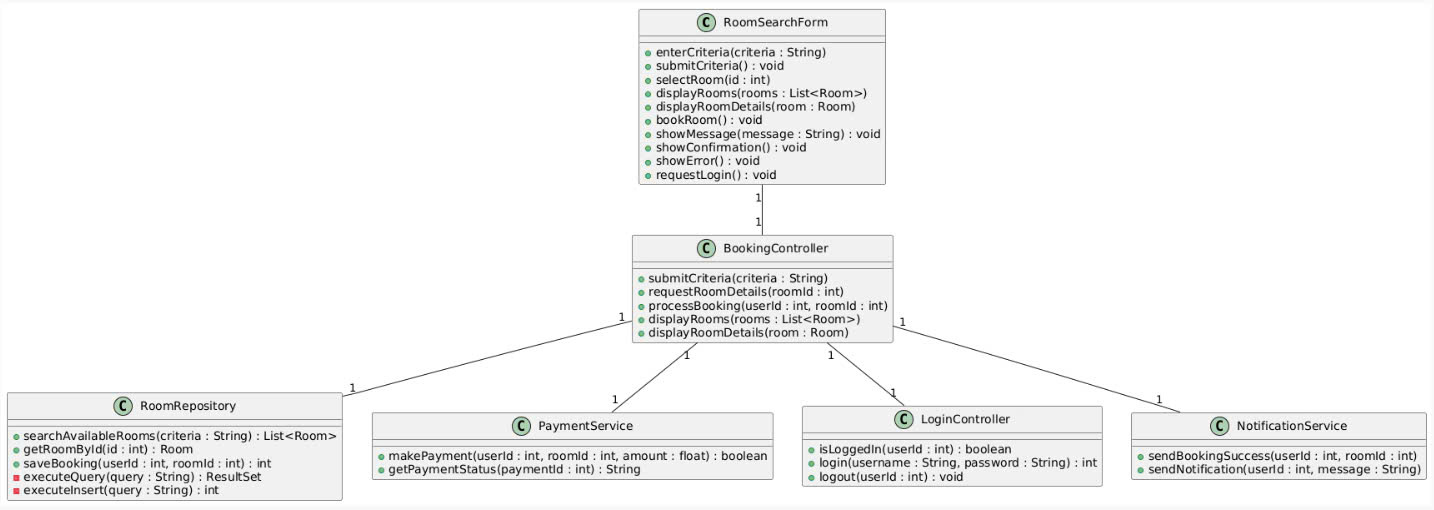
\includegraphics[width=\textwidth]{img3.4.2/thuephong4.jpg} 
    \caption{Biểu đồ lớp Đặt phòng khách sạn}
\end{figure}

\subsubsection{Theo dõi phòng đã đặt}
\begin{figure}[H]
    \centering
    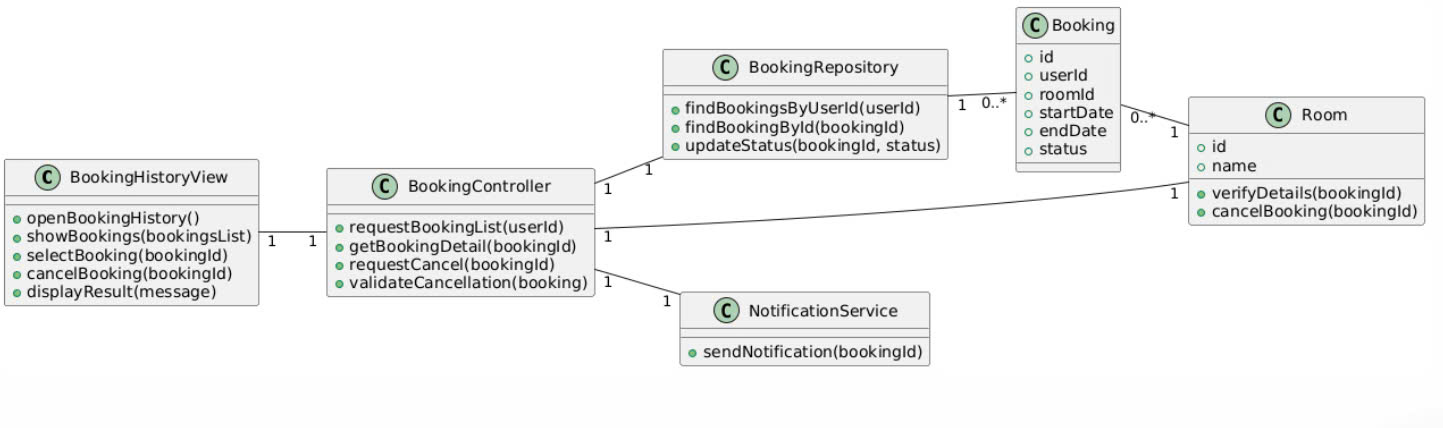
\includegraphics[width=\textwidth]{img3.4.2/xemphongthue4.jpg} 
    \caption{Biểu đồ lớp Theo dõi phòng đã đặt}
\end{figure}


\subsubsection{Đánh giá phòng đã thuê}
\begin{figure}[H]
    \centering
    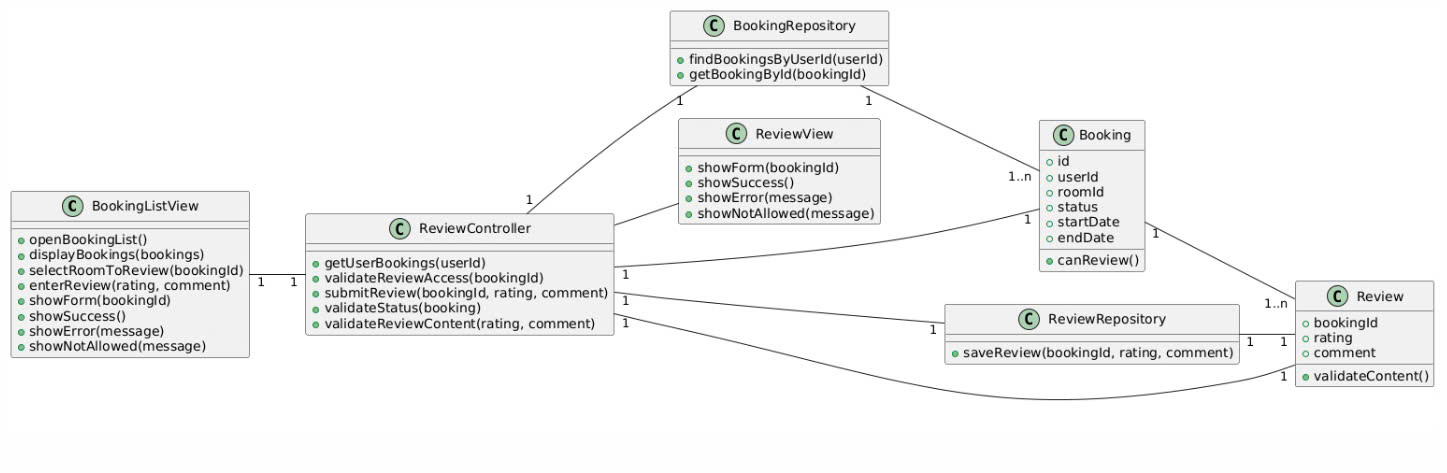
\includegraphics[width=\textwidth]{img3.4.2/dgia4.jpg} 
    \caption{Biểu đồ lớp Đánh giá phòng đã thuê}
\end{figure}


\subsubsection{Liên hệ với chủ khách sạn}
\begin{figure}[H]
    \centering
    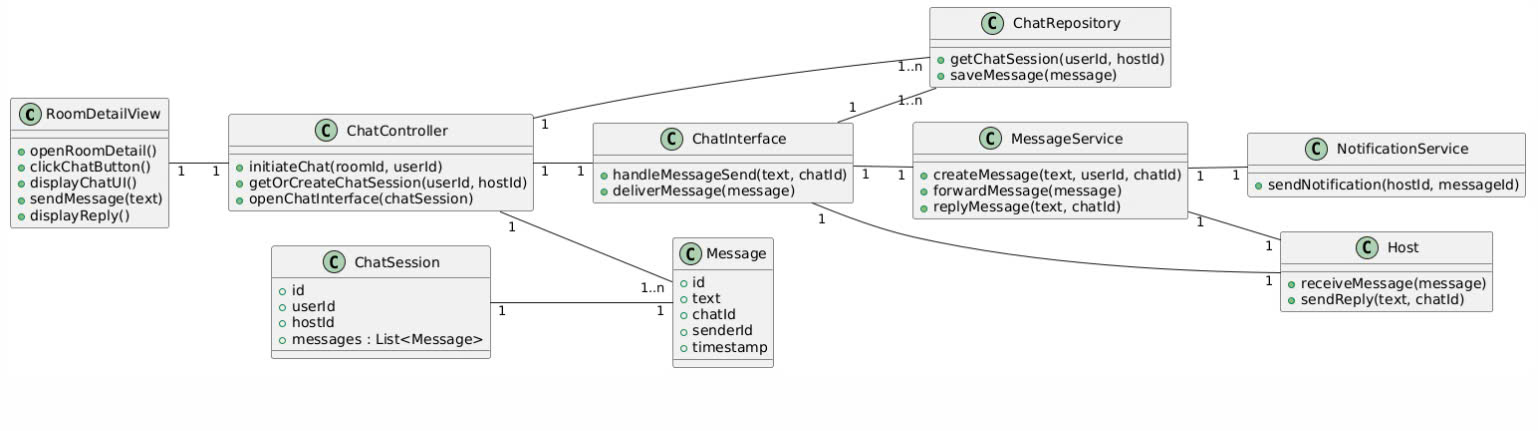
\includegraphics[width=\textwidth]{img3.4.2/chat4.jpg} 
    \caption{Biểu đồ lớp Liên hệ với chủ khách sạn}
\end{figure}

\subsubsection{Xem danh sách phòng yêu thích}
\begin{figure}[H]
    \centering
    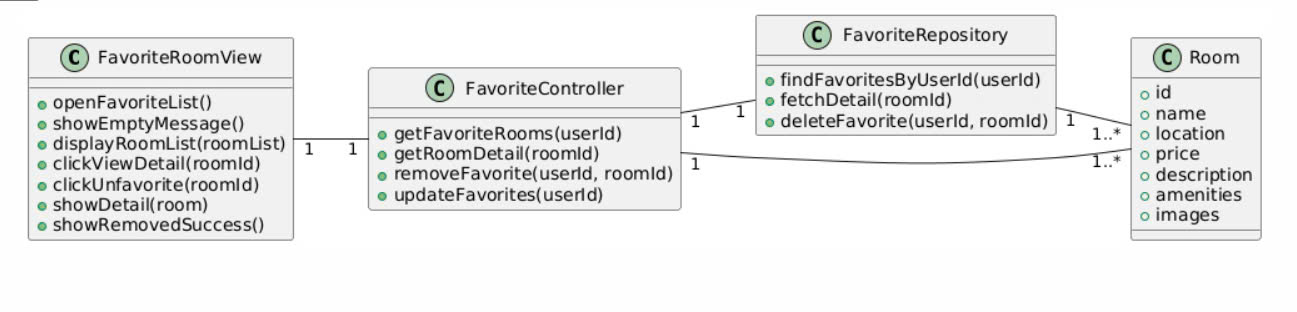
\includegraphics[width=\textwidth]{img3.4.2/xemphongyeu4.jpg} 
    \caption{Biểu đồ lớp Xem danh sách phòng yêu thích}
\end{figure}

\subsubsection{Cho thuê phòng}
\begin{figure}[H]
    \centering
    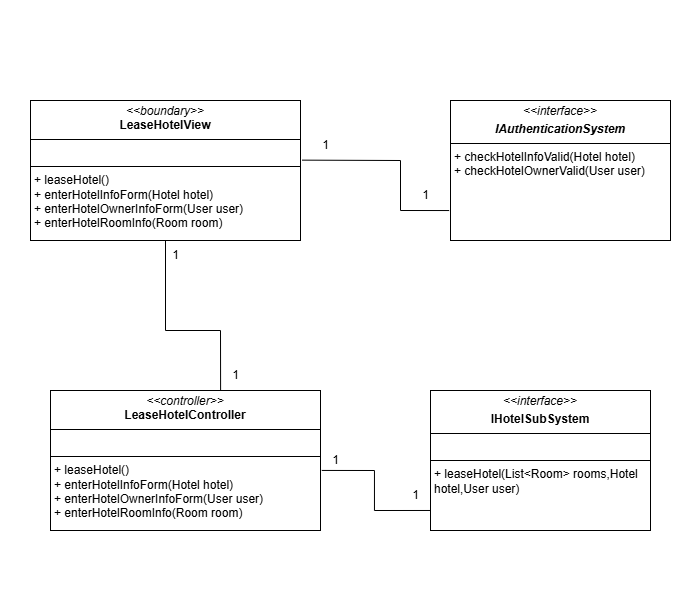
\includegraphics[width=0.7\textwidth]{img3.4.2/chothuephong.png} 
    \caption{Biểu đồ lớp Cho thuê phòng}
\end{figure}

\subsubsection{Sửa thông tin phòng}
\begin{figure}[H]
    \centering
    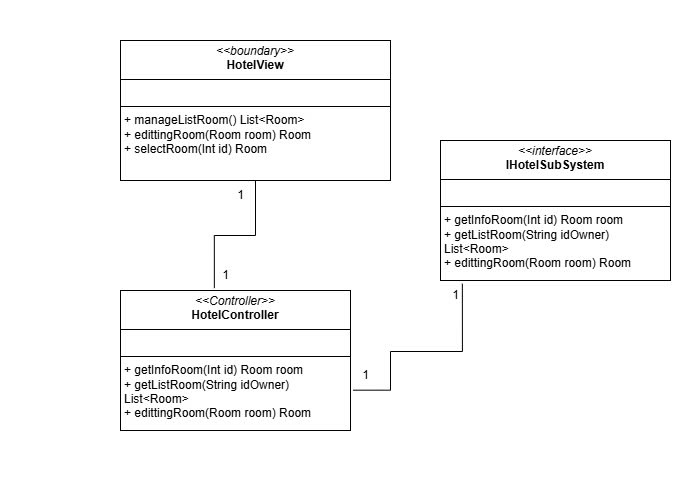
\includegraphics[width=0.55\textwidth]{img3.4.2/doithongtinphong.jpg} 
    \caption{Biểu đồ lớp Sửa thông tin phòng}
\end{figure}

\subsubsection{Tra cứu thông tin phòng đang cho thuê}
\begin{figure}[H]
    \centering
    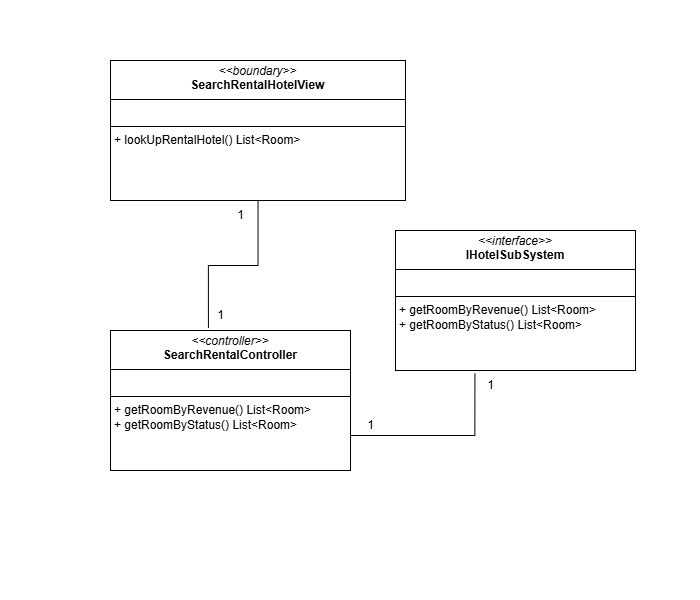
\includegraphics[width=\textwidth]{img3.4.2/tracuuphong.jpg} 
    \caption{Biểu đồ lớp Tra cứu thông tin phòng đang cho thuê}
\end{figure}

\subsubsection{Xóa phòng khách sạn}
\begin{figure}[H]
    \centering
    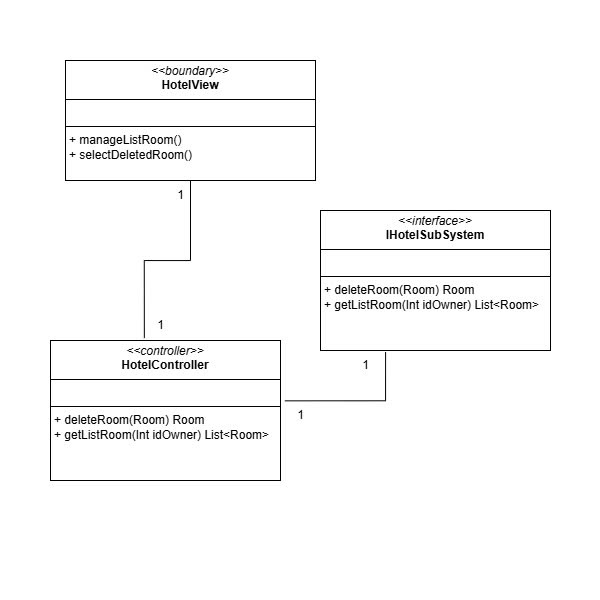
\includegraphics[width=0.8\textwidth]{img3.4.2/xoaphong.jpg} 
    \caption{Biểu đồ lớp Xóa phòng khách sạn}
\end{figure}

\subsubsection{Thanh toán}
\begin{figure}[H]
    \centering
    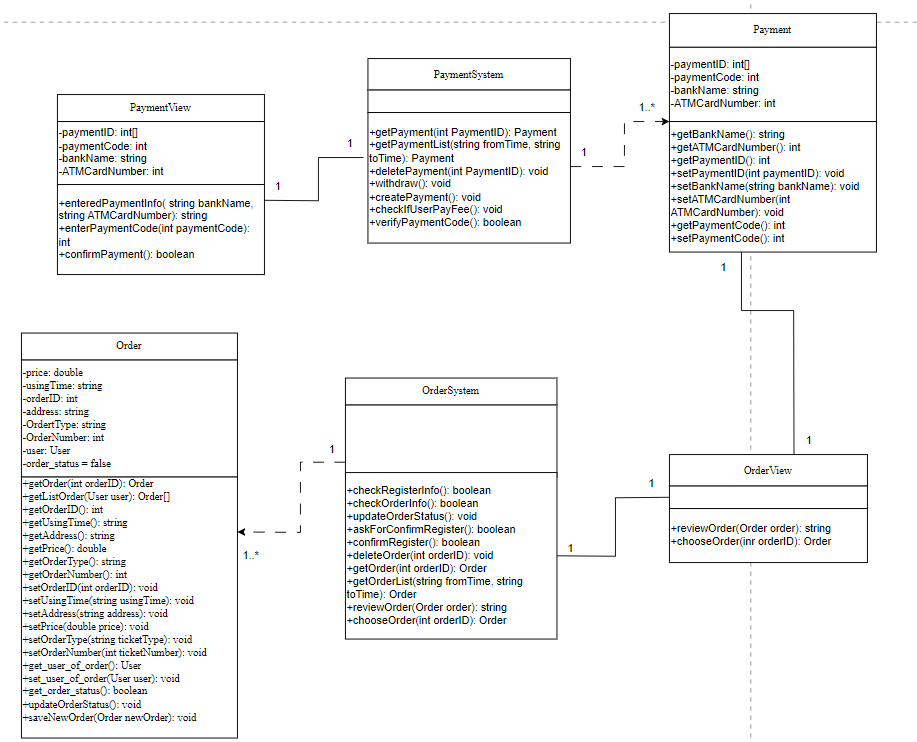
\includegraphics[width=\textwidth]{img3.4.2/3.4.2thanhtoanbangtk.png} 
    \caption{Biểu đồ lớp Thanh toán trực tuyến}
\end{figure}

\begin{figure}[H]
    \centering
    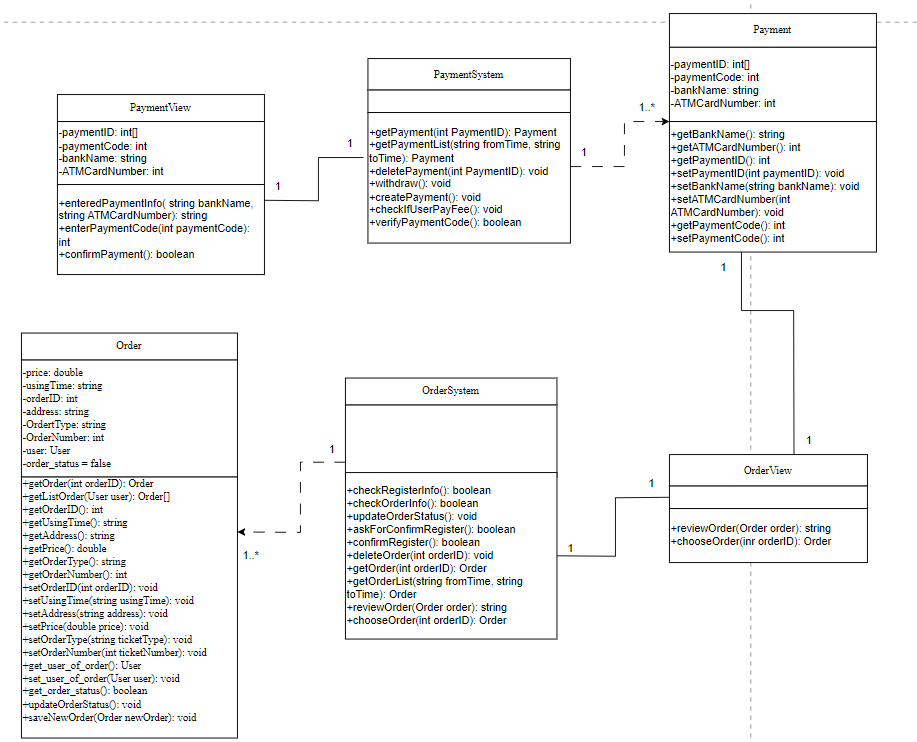
\includegraphics[width=\textwidth]{img3.4.2/3.4.2thanhtoantructiep.png} 
    \caption{Biểu đồ lớp Thanh toán trực tiếp}
\end{figure}

\subsubsection{Tra cứu phương tiện}
\begin{figure}[H]
    \centering
    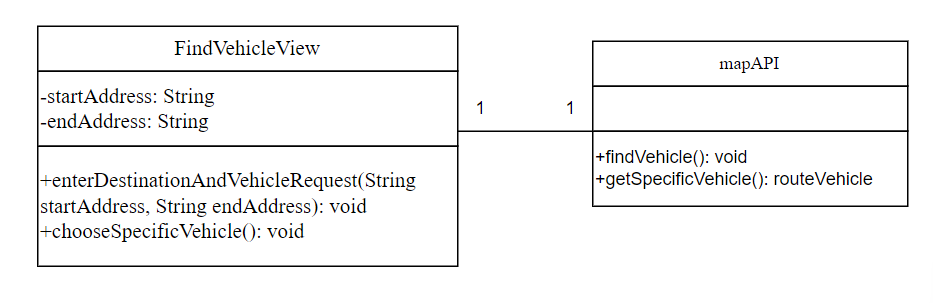
\includegraphics[width=\textwidth]{img3.4.2/3.4.2timphuongtien.png} 
    \caption{Biểu đồ lớp Tra cứu phương tiện}
\end{figure}

\subsubsection{Đăng ký tài khoản}
\begin{figure}[H]
    \centering
    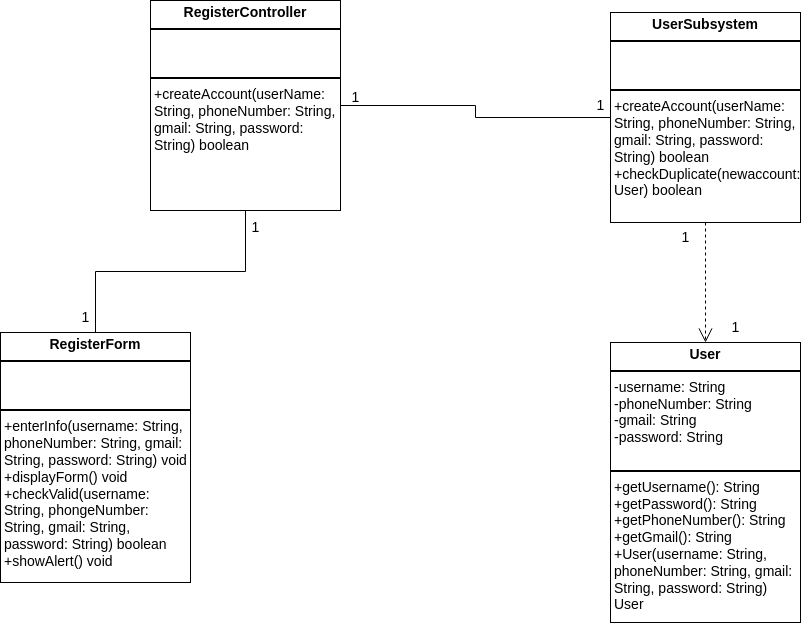
\includegraphics[width=\textwidth]{img3.4.2/Design_diagram-Lớp đăng ký.drawio.png} 
    \caption{Biểu đồ lớp Đăng ký tài khoản}
\end{figure}

\subsubsection{Đăng nhập}
\begin{figure}[H]
    \centering
    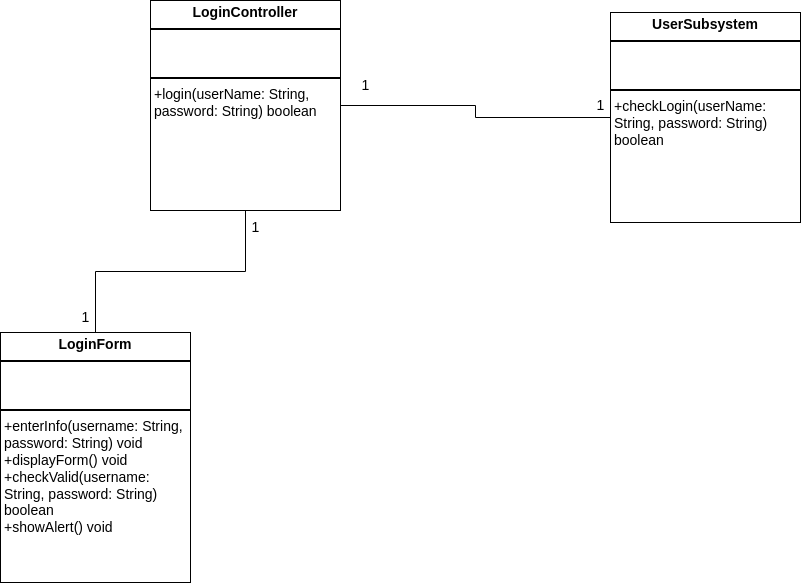
\includegraphics[width=0.9\textwidth]{img3.4.2/Design_diagram-Lớp đăng nhập.drawio.png} 
    \caption{Biểu đồ lớp Đăng nhập}
\end{figure}

\begin{figure}[H]
    \centering
    \includegraphics[width=0.9\textwidth]{img3.4.2/Design_diagram-Lớp quên mật khẩu.drawio.png} 
    \caption{Biểu đồ lớp Quên mật khẩu}
\end{figure}

\begin{figure}[H]
    \centering
    \includegraphics[width=\textwidth]{img3.4.2/Design_diagram-Lớp thay đổi thông tin.drawio.png} 
    \caption{Biểu đồ lớp Thay đổi thông tin tài khoản}
\end{figure}

\begin{figure}[H]
    \centering
    \includegraphics[width=\textwidth]{img3.4.2/Design_diagram-Lớp xóa tài khoản.drawio.png} 
    \caption{Biểu đồ lớp Xóa tài khoản}
\end{figure}

\subsubsection{Lựa chọn ngôn ngữ}
\begin{figure}[H]
    \centering
    \includegraphics[width=\textwidth]{img3.4.2/Design_diagram-Lớp chọn ngôn ngữ.drawio.png} 
    \caption{Biểu đồ lớp Lựa chọn ngôn ngữ}
\end{figure}

\section{Thiết kế Hệ thống con}
\subsection{User Subsystem}
\begin{figure}[H]
    \centering
    \includegraphics[width=\textwidth]{img3.5/user/cauTruc(UserSst).png} 
    \caption{Biểu đồ cấu trúc UserSubsystem}
\end{figure}

\begin{figure}[H]
    \centering
    \includegraphics[width=\textwidth]{img3.5/user/quanHe(UserSst).png} 
    \caption{Biểu đồ quan hệ UserSubsystem}
\end{figure}
\textbf{Interface IUserSubsystem}
    \begin{enumerate}
        \item Hàm changePassword()
        \begin{figure}[H]
        \centering
        \includegraphics[width=0.7\linewidth]{img3.5/user/changePassword.png}
        \end{figure}
        \item Hàm checkLogin()
        \begin{figure}[H]
        \centering
        \includegraphics[width=0.8\linewidth]{img3.5/user/checkLogin.png} 
        \end{figure}
        \item Hàm createAccount()
        \begin{figure}[H]
        \centering
        \includegraphics[width=0.75\linewidth]{img3.5/user/createAccount.png} 
        \end{figure}
        \item Hàm deleteUser()
        \begin{figure}[H]
        \centering
        \includegraphics[width=0.7\linewidth]{img3.5/user/deleteUser.png} 
        \end{figure}
        \item Hàm updateUser()
        \begin{figure}[H]
        \centering
        \includegraphics[width=0.875\linewidth]{img3.5/user/updateUser.png} 
        \end{figure}
        \item Hàm checkDuplicate()
        \begin{figure}[H]
        \centering
        \includegraphics[width=0.7\linewidth]{img3.5/user/checkDuplicate.png}
        \end{figure}
        \item Hàm verifyPaymentCode()
        \begin{figure}[H]
        \centering
        \includegraphics[width=0.7\linewidth]{img3.5/user/verifyPaymentCode.png}
        \end{figure}
    \end{enumerate}

\subsection{Hotel Subsystem}
\begin{figure}[H]
    \centering
    \includegraphics[width=\textwidth]{img3.5/hotel/hotelsubsystem1.drawio (1).png} 
    \caption{Biểu đồ cấu trúc HotelSubSystem}
\end{figure}

\begin{figure}[H]
    \centering
    \includegraphics[width=\textwidth]{img3.5/hotel/newHotelSub.png} 
    \caption{Biểu đồ quan hệ HotelSubSystem}
\end{figure}

\textbf{Interface IHotelSubsystem}
    \begin{enumerate}
        \item Hàm leaseHotel()
        \begin{figure}[H]
        \centering
        \includegraphics[width=0.8\linewidth]{img3.5/hotel/leaseHotel.jpg} 
        \end{figure}
        \item Hàm deleteRoom()
        \begin{figure}[H]
        \centering
        \includegraphics[width=0.8\linewidth]{img3.5/hotel/deleteRoom.png} 
        \end{figure}
        \item Hàm edittingRoomInfo()
        \begin{figure}[H]
        \centering
        \includegraphics[width=0.8\linewidth]{img3.5/hotel/edittingRoomInfo.png} 
        \end{figure}
        \item Hàm getRoomsByRenenue()
        \begin{figure}[H]
        \centering
        \includegraphics[width=0.8\linewidth]{img3.5/hotel/getRoomsByRenenue.png} 
        \end{figure}
        \item Hàm getRoomsByStatus()
        \begin{figure}[H]
        \centering
        \includegraphics[width=0.85\linewidth]{img3.5/hotel/getRoomByStatus.png} 
        \end{figure}
        \item Hàm bookingRoom()
        \begin{figure}[H]
        \centering
        \includegraphics[width=0.9\linewidth]{img3.5/hotel/newbookingRoom.png} 
        \end{figure}
        \item Hàm exchangeWithOwner()
        \begin{figure}[H]
        \centering
        \includegraphics[width=0.9\linewidth]{img3.5/hotel/exchangeWithOwner.png} 
        \end{figure}
        \item Hàm reviewRoom()
        \begin{figure}[H]
        \centering
        \includegraphics[width=0.95\linewidth]{img3.5/hotel/reviewRoom.png} 
        \end{figure}
        \item Hàm getBookedRoom()
        \begin{figure}[H]
        \centering
        \includegraphics[width=\linewidth]{img3.5/hotel/getBookedRoom.png} 
        \end{figure}
    \end{enumerate}

\section{Thiết kế lớp}
\begin{figure}[H]
    \centering
    \includegraphics[width=\linewidth]{img3.6/1.png}
\end{figure}
\begin{figure}[H]
    \centering
    \includegraphics[width=\linewidth]{img3.6/2.png}
\end{figure}
\begin{figure}[H]
    \centering
    \includegraphics[width=\linewidth]{img3.6/3.png}
\end{figure}
\begin{figure}[H]
    \centering
    \includegraphics[width=\linewidth]{img3.6/4.png}
\end{figure}
\begin{figure}[H]
    \centering
    \includegraphics[width=\linewidth]{img3.6/5.png}
\end{figure}
\begin{figure}[H]
    \centering
    \includegraphics[width=\linewidth]{img3.6/6.png}
\end{figure}
\begin{figure}[H]
    \centering
    \includegraphics[width=\linewidth]{img3.6/7.png}
\end{figure}
\begin{figure}[H]
    \centering
    \includegraphics[width=\linewidth]{img3.6/8.png}
\end{figure}
\begin{figure}[H]
    \centering
    \includegraphics[width=\linewidth]{img3.6/9.png}
\end{figure}
\begin{figure}[H]
    \centering
    \includegraphics[width=\linewidth]{img3.6/10.png}
\end{figure}
\begin{figure}[H]
    \centering
    \includegraphics[width=0.8\linewidth]{img3.6/11.png}
\end{figure}
\begin{figure}[H]
    \centering
    \includegraphics[width=0.8\linewidth]{img3.6/12.png}
\end{figure}
\begin{figure}[H]
    \centering
    \includegraphics[width=\linewidth]{img3.6/13.png}
\end{figure}
\begin{figure}[H]
    \centering
    \includegraphics[width=\linewidth]{img3.6/14.png}
\end{figure}

\section{Thiết kế Cơ sở dữ liệu}
\begin{figure}[H]
    \centering
    \includegraphics[width=\linewidth]{img3.7/3.7.png}
\end{figure}

\textbf{Bảng phân chia công việc}
\begin{longtable}{
    |p{1cm}
    |>{\raggedright\arraybackslash}p{3.5cm}
    |>{\raggedright\arraybackslash}p{3.5cm}
    |>{\raggedright\arraybackslash}p{3.5cm}
    |>{\raggedright\arraybackslash}p{3.5cm}|
}
\hline
 & Phạm Đức Thiện & Phạm Tuấn Việt & Đoàn Văn Tuyến & Phạm Văn Minh \\
\hline
Đặc tả & +Đặt vấn đề\newline 
        +Bảng thuật ngữ\newline 
        +Đặc tả bổ sung\newline 
        +Sơ đồ Usecase\newline
        +Đặc tả Đăng ký tài khoản\newline
        +Đặc tả Đăng nhập\newline
        +Đặc tả Lựa chọn ngôn ngữ\newline
       & +Đặc tả Cho thuê phòng\newline
       +Đặc tả Sửa thông tin phòng\newline
       +Đặc tả Tra cứu thông tin phòng đang cho thuê\newline
       +Đặc tả Xóa phòng khách sạn\newline
       & +Đặc tả Đặt phòng khách sạn\newline +Đặc tả Theo dõi phòng đã đặt\newline +Đặc tả Đánh giá phòng đã thuê\newline
       +Đặc tả Liên hệ với chủ khách sạn\newline
       +Đặc tả Xem danh sách phòng yêu thích\newline
       &+Đặc tả Thanh toán\newline
       +Đặc tả Tra cứu phương tiện\newline
\\
\hline
Phân tích 
&+Phân tích kiến trúc\newline
+Biểu đồ lớp, tuần tự Đăng ký tài khoản\newline
+Biểu đồ lớp, tuần tự Đăng nhập\newline
+Biểu đồ lớp, tuần tự Lựa chọn ngôn ngữ\newline
+Ánh xạ từ lớp phân tích tới cơ chế phân tích\newline
&+Biểu đồ lớp, tuần tự Cho thuê phòng\newline
+Biểu đồ lớp, tuần tự Chỉnh sửa thông tin phòng khách sạn\newline
+Biểu đồ lớp, tuần tự Tra cứu thông tin phòng cho thuê\newline
+Biểu đồ lớp, tuần tự Xóa phòng khách sạn\newline
&+Biểu đồ lớp, tuần tự Đặt phòng khách sạn\newline
+Biểu đồ lớp, tuần tự Theo dõi phòng đã đặt\newline
+Biểu đồ lớp, tuần tự Đánh giá phòng đã thuê\newline
+Biểu đồ lớp, tuần tự Liên hệ với chủ khách sạn\newline
+Biểu đồ lớp, tuần tự Xem danh sách phòng yêu thích\newline
&+Biểu đồ lớp, tuần tự Thanh toán\newline
+Biểu đồ lớp, tuần tự  Tra cứu phương tiện\newline
\\
\hline
Thiết kế
&+Analysis-to-Design-to-Implementation Mechanisms Map\newline
+Analysis-Class-to-Design-Element Map\newline
+Design-Element-to-Owning-Package Map\newline
+Biểu đồ lớp, tuần tự Đăng ký tài khoản\newline
+Biểu đồ lớp, tuần tự Đăng nhập\newline
+Biểu đồ lớp, tuần tự Lựa chọn ngôn ngữ\newline
&+Subsystem Context\newline
+Biểu đồ lớp, tuần tự Cho thuê phòng\newline
+Biểu đồ lớp, tuần tự Chỉnh sửa thông tin phòng khách sạn\newline
+Biểu đồ lớp, tuần tự Tra cứu thông tin phòng cho thuê\newline
+Biểu đồ lớp, tuần tự Xóa phòng khách sạn\newline
+Thiết kế Hệ thống con\newline
&+Packages and Their Dependency\newline
+Mô tả kiến trúc thực thi\newline
+Biểu đồ lớp, tuần tự Đặt phòng khách sạn\newline
+Biểu đồ lớp, tuần tự Theo dõi phòng đã đặt\newline
+Biểu đồ lớp, tuần tự Đánh giá phòng đã thuê\newline
+Biểu đồ lớp, tuần tự Liên hệ với chủ khách sạn\newline
+Biểu đồ lớp, tuần tự Xem danh sách phòng yêu thích\newline
&+Biểu đồ lớp, tuần tự Thanh toán\newline
+Biểu đồ lớp, tuần tự  Tra cứu phương tiện\newline
+Thiết kế lớp\newline
+Thiết kế Cơ sở dữ liêu\newline
\\
\hline
Hệ số&25\%&25\%&25\%&25\%
\\
\hline
\end{longtable}
